\documentclass{cskkuproject}

% ==========================================
% ข้อมูลโครงงาน — ตัวอย่างประเภท A: พัฒนาระบบ
% ==========================================

\titleTH{การออกแบบและพัฒนาเกมเดินเรือด้วยระบบสั่งการด้วยเสียงเพื่อส่งเสริมทักษะการสื่อสาร}
\titleEN{Design and Development of a Voice-Controlled Ship Navigation Game to Enhance Communication Skills}

% ข้อมูลนักศึกษาคนที่ 1
\firstStudentID{663380213-6}
\firstStudentPrefixTH{นาย}
\firstStudentPrefixEN{Mr.}
\firstStudentNameTH{ธิติวุฒิ ศรีอมรรัตน์}
\firstStudentNameEN{Thitiwut Sriamonrat}

% ข้อมูลหลักสูตร
\degreeTH{วิทยาศาสตรบัณฑิต}
\degreeEN{Bachelor of Science}
\majorTH{วิทยาการคอมพิวเตอร์}
\majorEN{Computer Science}

% อาจารย์ที่ปรึกษา
\advisorTH{ผศ.ดร.วชิราวุธ ธรรมวิเศษ}
\advisorEN{Asst.Prof.Wachirawut Thamviset, Ph.D.}

% ปีการศึกษา
\academicYearTH{2569}
\academicYearEN{2026}

% รหัสวิชา
\courseCode{CP354 771}
\courseName{โครงงานทางวิทยาการคอมพิวเตอร์}
\semester{2}

% คำสำคัญ
\keywordsTH{เกมผู้เล่นเดี่ยว, เกม 3 มิติ, การรู้จำเสียง, เกมเดินเรือ, Gamification, Digital Game-Based Learning}
\keywordsEN{Single-player game, 3D game, Speech recognition, Ship navigation game, Gamification, Digital Game-Based Learning}


\begin{document}

% ==========================================
% หน้าปก
% ==========================================
\maketitlepage

% ตั้งค่าเลขหน้าส่วนต้นเป็นอักษรไทย (ก, ข, ค, ...)
\pagenumbering{arabic}
\setcounter{page}{0}
\renewcommand{\thepage}{\ThaiAlph{\value{page}}}

% ==========================================
% บทคัดย่อ
% ==========================================
\begin{abstractTH}
% บทคัดย่อภาษาไทย
โครงงานฉบับนี้มีวัตถุประสงค์เพื่อออกแบบและพัฒนาเกมเดินเรือด้วยระบบสั่งการด้วยเสียง (Voice-Controlled Ship Navigation Game) สำหรับเป็นสื่อการเรียนรู้เพื่อส่งเสริมทักษะการสื่อสารและลดความวิตกกังวลในการใช้ภาษาต่างประเทศของผู้เรียน โดยระบบผสมผสานรูปแบบเกมจำลองสถานการณ์เข้ากับเทคโนโลยีการรู้จำเสียง (Speech Recognition) ประกอบด้วย 5 ระบบหลัก ได้แก่ ระบบรับคำสั่งเสียงและการประมวลผลคำสั่ง ระบบฟิสิกส์และการควบคุมยานพาหนะ ระบบลูกเรือปัญญาประดิษฐ์ ระบบสุ่มสร้างสิ่งกีดขวาง และระบบอินเทอร์เฟซผู้ใช้ รองรับผู้ใช้ในบทบาทกัปตันเรือ (ผู้เล่น) ที่ต้องสื่อสารและสั่งการลูกเรือปัญญาประดิษฐ์ ได้แก่ พลต้นหนและพลถือท้าย ระบบพัฒนาด้วยเอนจิน Unity 3D และภาษา C\# สำหรับโครงสร้างเกม และใช้เทคโนโลยีประมวลผลภาษาธรรมชาติร่วมกับโมเดลการรู้จำเสียงอย่าง Whisper AI สำหรับแปลงคำสั่งเสียงภาษาอังกฤษเป็นข้อความเพื่อประมวลผล ระบบลูกเรือปัญญาประดิษฐ์ช่วยให้เกิดการจำลองสถานการณ์สื่อสารขัดข้องเมื่อผู้เล่นออกเสียงไม่ชัดเจนหรือใช้คำสั่งผิดบริบท โดยลูกเรือจะทวนถามหรือขอให้ย้ำคำสั่งได้โดยตรง ทำให้การฝึกความคล่องแคล่วในการพูดและการแก้ปัญหาเฉพาะหน้าภายใต้ความกดดันมีประสิทธิภาพยิ่งขึ้น โดยจะมีการวัดผลการทดสอบและประเมินประสิทธิภาพผ่านแบบประเมินจากกลุ่มผู้ทดสอบจำนวน 40-50 คน
\end{abstractTH}

\begin{abstractEN}
% ABSTRACT (English)
This project aims to design and develop a Voice-Controlled Ship Navigation Game as a learning tool to enhance communication skills and reduce foreign language anxiety among learners. The system integrates a simulation game format with Speech Recognition technology and consists of five main systems: the voice command reception and processing system, the ship physics and control system, the AI crew system, the random obstacle generation system, and the user interface. It supports the user in the role of a ship captain (the player) who must communicate with and issue commands to an AI crew, specifically the navigator and the helmsman. The game is developed using the Unity 3D engine and C\#, utilizing natural language processing alongside a speech recognition model such as Whisper AI to convert English voice commands into text for processing. The AI crew system enables the simulation of communication breakdowns; if the player's pronunciation is unclear or a command is out of context, the crew will directly request clarification or repetition. This effectively enhances speaking fluency and real-time problem-solving skills under pressure. The system's performance and user experience will be evaluated using assessment forms from a test group of 40-50 participants.

\end{abstractEN}

% ==========================================
% กิตติกรรมประกาศ
% ==========================================
\begin{acknowledgement}
ข้าพเจ้าขอขอบพระคุณ ผศ.ดร.วชิราวุธ ธรรมวิเศษ อาจารย์ที่ปรึกษาโครงงาน
ที่ได้กรุณาให้คำแนะนำ คำปรึกษา และข้อเสนอแนะอันเป็นประโยชน์
รวมทั้งสละเวลาในการตรวจแก้ไข

ขอขอบพระคุณเพื่อนร่วมชั้นและผู้ที่เกี่ยวข้องทุกท่าน
ที่ได้ให้ความช่วยเหลือ แนะนำ และแลกเปลี่ยนความคิดเห็น
ซึ่งเป็นประโยชน์ต่อการดำเนินงานในหลายด้าน

ท้ายที่สุดนี้ ข้าพเจ้าขอขอบพระคุณบิดา มารดา และครอบครัว
ที่ให้การสนับสนุน ส่งเสริม ตลอดระยะเวลาของการศึกษา

\end{acknowledgement}

% ==========================================
% สารบัญ
% ==========================================
\tableofcontents
\clearpage
\listoffigures
\clearpage
\listoftables
\clearpage

% ==========================================
% เนื้อเรื่อง 5 บท
% ==========================================
\pagenumbering{arabic}
\setcounter{page}{1}

\chapter{บทนำ}
% =============================================================
% บทที่ 1 - บทนำ
% โครงงาน: การออกแบบและพัฒนาเกมเดินเรือด้วยระบบสั่งการด้วยเสียงเพื่อส่งเสริมทักษะการสื่อสาร
%          (Design and Development of a Voice-Controlled Ship Navigation Game to Enhance Communication Skills)
% =============================================================

% -----------------------------------------------------------
\section{ความเป็นมาและความสำคัญของปัญหา}
% -----------------------------------------------------------
ในปัจจุบัน ภาษาอังกฤษมีบทบาทสำคัญอย่างยิ่งในการเป็นเครื่องมือสื่อสารระดับสากล ทว่าการเรียนการสอนภาษาอังกฤษในห้องเรียนโดยทั่วไปยังคงเผชิญกับข้อจำกัดในการสร้างสภาพแวดล้อมที่เอื้อต่อการนำไปใช้งานจริง\cite{sadigzade2025} ผู้เรียนจำนวนมากประสบปัญหาความวิตกกังวล (Language Anxiety) และกลัวความผิดพลาดเมื่อต้องเปล่งเสียงเพื่อสื่อสาร ส่งผลให้ขาดความมั่นใจและไม่สามารถเชื่อมโยงทักษะทางภาษาเข้ากับสถานการณ์ในชีวิตจริงหรือการโต้ตอบแบบทันท่วงทีได้\cite{varma2025} 
ที่ผ่านมา มีความพยายามนำสื่อดิจิทัลและเกมมาประยุกต์ใช้เพื่อการเรียนรู้ภาษา (Game-Based Language Learning) แต่ยังคงพบกับความท้าทายสำคัญ\cite{sadigzade2025, sanchez2010, allain2015} งานวิจัยชี้ให้เห็นว่าแอปพลิเคชันหรือเกมเพื่อการเรียนรู้ภาษาแบบดั้งเดิมมักมีความหนาแน่นทางไวยากรณ์และการท่องจำคำศัพท์ ทำให้รูปแบบการเล่นจำเจอยู่กับการคลิกเลือกคำตอบหรือการอ่านข้อความ ในขณะที่เกมที่เน้นความสนุกสนานก็มักไม่ได้บังคับให้ผู้เล่นต้องเปล่งเสียงพูดออกมาจริง ๆ\cite{varma2025} ช่องว่างนี้แสดงให้เห็นถึงโอกาสในการสร้างสรรค์เกมที่สามารถบูรณาการการฝึกฝนทักษะการพูดเข้ากับบริบทที่น่าตื่นเต้นและท้าทาย เพื่อกระตุ้นให้เกิดการสื่อสารอย่างเป็นธรรมชาติ\cite{zargham2024}
โครงงานการออกแบบและพัฒนาเกมเดินเรือด้วยระบบสั่งการด้วยเสียงเพื่อส่งเสริมทักษะการสื่อสารจึงถูกนำเสนอขึ้น เพื่อพัฒนาแนวทางการเรียนรู้ภาษาอังกฤษผ่านสภาพแวดล้อมเสมือนจริง (Immersive Environment) ผู้เล่นจะรับบทเป็น "กัปตันเรือ" ที่ต้องเผชิญกับสถานการณ์จำลองการเดินเรือฝ่าสภาพแวดล้อมที่ท้าทาย โดยภารกิจของผู้เล่นไม่ใช่เพียงการควบคุมทิศทางผ่านหน้าจอ แต่คือการใช้ "เสียง" เป็นเครื่องมือหลักในการควบคุมและสั่งการลูกเรือปัญญาประดิษฐ์ (AI Crew) ในตำแหน่งต่าง ๆ เช่น พลต้นหน (Navigator) และพลถือท้ายเรือ (Helmsman) เพื่อบังคับเรือไม่ให้ชนสิ่งกีดขวางและนำเรือไปสู่เป้าหมายอย่างปลอดภัย

% -----------------------------------------------------------
\section{นิยามศัพท์เฉพาะ}
% -----------------------------------------------------------

\begin{enumerate}[label=\arabic*)]
    \item \textbf{เกมเพื่อการเรียนรู้ (Serious Game)} หมายถึง เกมแนวจำลองสถานการณ์ที่ถูกออกแบบมาเพื่อใช้เป็นสื่อการเรียนรู้แบบดื่มด่ำ (Immersive Learning) ที่มีความสมจริง
    \item \textbf{การรู้จำเสียง (Speech-to-Text / Speech Recognition)} หมายถึง เทคโนโลยีการแปลงคำสั่งเสียงพูดภาษาอังกฤษของผู้เล่นให้เป็นข้อความ เพื่อนำไปตรวจความถูกต้องและประมวลผลเป็นคำสั่งควบคุมเรือ
    \item \textbf{ตัวกรองทางอารมณ์ (Affective Filter)} หมายถึง อุปสรรคทางอารมณ์ เช่น ความกลัว ความวิตกกังวล และความขาดความมั่นใจ ซึ่งขัดขวางการเรียนรู้และการพูดภาษาที่สอง
    \item \textbf{ลูกเรือปัญญาประดิษฐ์ (AI Crew)} หมายถึง ตัวละคร NPC (Non-Player Character) ในเกมที่รับคำสั่งเสียงจากผู้เล่นและให้เสียงตอบกลับ (Voice Feedback) เช่น การทวนคำสั่งหรือขอให้ย้ำคำสั่ง
    \item \textbf{สภาพแวดล้อมเสมือนจริง (Immersive Environment)} หมายถึง สภาพแวดล้อมจำลองภายในเกมที่สร้างประสบการณ์การเรียนรู้ที่มีทั้งความท้าทาย ความสมจริง และความปลอดภัยทางความรู้สึก
\end{enumerate}

% -----------------------------------------------------------
\section{วัตถุประสงค์}
% -----------------------------------------------------------

\begin{enumerate}[label=\arabic*)]
    \item เพื่อออกแบบและพัฒนาเกมเดินเรือด้วยระบบสั่งการด้วยเสียง (Voice-Controlled Ship Navigation Game) สำหรับใช้เป็นสื่อการเรียนรู้แบบดื่มด่ำ (Immersive Learning) ที่มีความสมจริงและช่วยลดความวิตกกังวลในการใช้ภาษาต่างประเทศของผู้เรียน
    \item เพื่อประเมินประสิทธิภาพของระบบและประเมินความพึงพอใจของผู้ใช้งาน โดยศึกษาความแม่นยำและความหน่วง (Latency) ของระบบปัญญาประดิษฐ์ในเกม รวมถึงประเมินผลสัมฤทธิ์ด้านประสบการณ์การใช้งานของผู้เล่นที่มีต่อการใช้เกมเป็นสื่อเพื่อการเรียนรู้ภาษา
\end{enumerate}

% -----------------------------------------------------------
\section{เป้าหมายและขอบเขต}
% -----------------------------------------------------------

\subsection{ขอบเขตด้านเนื้อหา}

ระบบที่พัฒนาเป็นเกมแนวจำลองสถานการณ์ (Simulation Game) แบบผู้เล่นคนเดียว (Single-player) ที่ใช้เสียงเป็นอุปกรณ์ควบคุมหลัก ครอบคลุมการทำงาน 5 ระบบหลัก ดังนี้

\begin{enumerate}[label=\arabic*)]
    \item \textbf{ระบบรู้จำเสียงและการประมวลผลคำสั่ง (Speech Recognition \& Command Parser System):} ระบบรับเสียงจากไมโครโฟน แปลงเป็นข้อความ และตรวจสอบความถูกต้องของคำสั่งภาษาอังกฤษ
    \item \textbf{ระบบฟิสิกส์และการควบคุมยานพาหนะ (Ship Navigation Physics):} ระบบจำลองการเคลื่อนที่ของเรือที่มีความเฉื่อยและการตอบสนองต่อพวงมาลัยที่สมจริง ทำให้ผู้เล่นต้องวางแผนล่วงหน้าในการออกคำสั่ง
    \item \textbf{ระบบลูกเรือปัญญาประดิษฐ์ (AI Crew System):} ระบบตัวละคร NPC ที่รับคำสั่งเสียงจากผู้เล่นและให้เสียงตอบกลับ เช่น การทวนคำสั่งเมื่อรับทราบ หรือการแจ้งเตือนเมื่อไม่เข้าใจคำสั่ง
    \item \textbf{ระบบสุ่มสร้างสิ่งกีดขวาง (Obstacle Generation System):} ระบบสร้างสิ่งกีดขวางแบบสุ่มในเส้นทางการเดินเรือ เพื่อท้าทายให้ผู้เล่นต้องตัดสินใจออกคำสั่งหลบหลีกในทันที
    \item \textbf{ระบบอินเทอร์เฟซผู้ใช้ (UI/HUD):} หน้าจอแสดงข้อมูลที่จำเป็น เช่น เรดาร์ตรวจจับสิ่งกีดขวาง เข็มทิศแสดงองศาเรือ มาตรวัดความเร็ว และสัญลักษณ์แสดงสถานะการรับเสียงของไมโครโฟน
\end{enumerate}

\subsection{ขอบเขตด้านประชากรและกลุ่มตัวอย่าง}

ทำการประเมินผลกับกลุ่มเป้าหมายคือนักศึกษาระดับปริญญาตรี หรือผู้ที่สนใจในการเรียนรู้และฝึกฝนทักษะการสื่อสารภาษาอังกฤษเบื้องต้นผ่านสื่อเกมแบบจำลองสถานการณ์ จำนวนกลุ่มผู้ทดลองประมาณ 40–50 คน

\subsection{ขอบเขตด้านเทคนิค}

\begin{enumerate}[label=\arabic*)]
    \item พัฒนาตัวเกมด้วย Game Engine Unity 3D และใช้ภาษา C\# สำหรับการพัฒนาสภาพแวดล้อมเกมและระบบฟิสิกส์ของการเดินเรือ
    \item นำเสนอภาพในรูปแบบมุมมองการเล่นแบบไอโซเมตริก (Isometric view) และรองรับการทำงานบนระบบปฏิบัติการ Windows PC
    \item ใช้ไมโครโฟนเป็นอุปกรณ์รับข้อมูล (Input) เสียงพูดภาษาอังกฤษ เป็นวิธีการหลักในการควบคุมทิศทางและความเร็วของเรือ โดยไม่มีการใช้คีย์บอร์ดหรือเมาส์ในการบังคับทิศทางโดยตรง
    \item ใช้ API หรือไลบรารีสำหรับการประมวลผลเสียง (Whisper) เพื่อแปลงเสียงพูดของผู้เล่นเป็นข้อความคำสั่ง (Text Parsing)
    \item ใช้บริการเชื่อมต่อระบบประมวลผล (API) สำหรับปัญญาประดิษฐ์ (OpenAI GPT-4o mini) เพื่อใช้ในระบบโต้ตอบและประมวลผลคำสั่งลูกเรือ
\end{enumerate}

% -----------------------------------------------------------
\section{ประโยชน์ที่คาดว่าจะได้รับ}
% -----------------------------------------------------------

\begin{enumerate}[label=\arabic*)]
    \item ผู้เล่นได้รับทักษะพื้นฐานด้านการสื่อสารภาษาอังกฤษและคำศัพท์ที่เกี่ยวข้องกับการเดินเรือ
    \item ผู้เล่นได้เกิดความมั่นใจในการพูดกล้าพูดภาษาอังกฤษมากยิ่งขึ้น
    \item สามารถนำไปใช้เป็นสื่อการสอนเพื่อส่งเสริมการเรียนรู้เชิงปฏิบัติ
\end{enumerate}

\chapter{ทฤษฎีและงานวิจัยที่เกี่ยวข้อง}
% =============================================================
% บทที่ 2 - งานวิจัยและทฤษฎีที่เกี่ยวข้อง
% โครงงาน: การออกแบบและพัฒนาเกมเดินเรือด้วยระบบสั่งการด้วยเสียงเพื่อส่งเสริมทักษะการสื่อสาร
% =============================================================

% -----------------------------------------------------------
\section{งานวิจัย โครงงาน และระบบงานที่เกี่ยวข้อง}
% -----------------------------------------------------------

ในส่วนนี้จะนำเสนอทฤษฎี งานวิจัย และเกมที่มีลักษณะคล้ายคลึงกับโครงงานนี้ เพื่อศึกษาแนวคิด จุดเด่น และข้อจำกัด แล้วนำมาเป็นแนวทางในการออกแบบและพัฒนาระบบ

\subsection{การเรียนรู้ภาษาผ่านเกมด้วยเทคโนโลยีการประมวลผลภาษาธรรมชาติ}

งานวิจัยของ Sadigzade\cite{sadigzade2025} นำเสนอการใช้เกมดิจิทัลร่วมกับเทคโนโลยีการรู้จำเสียงและการประมวลผลภาษาธรรมชาติ เพื่อสนับสนุนการเรียนรู้ภาษาอังกฤษ การให้ผู้เรียนได้โต้ตอบด้วยเสียงกับตัวละคร AI ภายในเกมช่วยสร้างสภาพแวดล้อมจำลองที่สมจริง ผลการศึกษาพบว่าช่วยเพิ่มแรงจูงใจ ลดความวิตกกังวลในการพูด และพัฒนาความคล่องแคล่วในการสื่อสารได้อย่างมีประสิทธิภาพ อย่างไรก็ตาม เกมในลักษณะดังกล่าวมักไม่ได้เน้นความกดดันด้านเวลาหรือสถานการณ์จำลองที่ต้องใช้ไหวพริบอย่างรวดเร็ว

\subsection{เครื่องมือเกมควบคุมด้วยเสียงเพื่อเสริมสร้างการเรียนรู้}

งานวิจัยของ Varma และคณะ\cite{varma2025} มุ่งเน้นพัฒนาเกมที่ควบคุมการทำงานด้วยคำสั่งเสียงแบบเรียลไทม์ โดยทำงานผ่านการแปลงเสียงพูดเป็นคำสั่งเพื่อควบคุมการเคลื่อนที่ขององค์ประกอบในเกมแทนการใช้อุปกรณ์ควบคุมปกติ การควบคุมผ่านเสียงช่วยกระตุ้นให้ผู้เล่นต้องคิดตัดสินใจอย่างรวดเร็วและเปล่งเสียงให้ชัดเจน ซึ่งช่วยพัฒนาทักษะการตอบสนองได้ดี

\subsection{การสำรวจการโต้ตอบด้วยเสียงกับตัวละคร NPC ในเกม}

Zargham และคณะ\cite{zargham2024} ได้สำรวจความคิดเห็นของผู้เชี่ยวชาญเกี่ยวกับการใช้เสียงพูดเพื่อสื่อสารกับตัวละคร NPC ในวิดีโอเกม ผลการวิจัยระบุว่าการสั่งการด้วยเสียงช่วยเพิ่มความรู้สึกดื่มด่ำ (Immersion) และความสมจริง นอกจากนี้ การให้ NPC ตอบสนองต่อคำสั่งเสียงอย่างเป็นธรรมชาติยังช่วยเพิ่มความผูกพันได้ แต่จำเป็นต้องคำนึงถึงบริบทและความแม่นยำของระบบรู้จำเสียงเพื่อป้องกันความหงุดหงิดจากการแปลความหมายผิดพลาด

\subsection{เกมจำลองการควบคุมยานพาหนะด้วยเสียง (Commercial Games)}

ในอุตสาหกรรมเกมเชิงพาณิชย์ ได้มีการนำระบบรู้จำเสียงมาใช้เพื่อเพิ่มความสมจริงในเกมแนวจำลองสถานการณ์ (Simulation) เช่น เกม Powerboat VR\cite{powerboat2020} ที่ผู้เล่นสามารถใช้คำสั่งเสียงภาษาอังกฤษในการควบคุมทิศทางและความเร็วของเรือแทนคอนโทรลเลอร์ปกติ หรือเกม Tower! 3D\cite{tower3d2017} ที่ผู้เล่นต้องใช้เสียงพูดตามมาตรฐานคำศัพท์การบินเพื่อสั่งการเครื่องบิน เกมเหล่านี้แสดงให้เห็นว่าคำสั่งเสียงสามารถสร้างประสบการณ์ที่ดื่มด่ำได้เป็นอย่างดี

\subsection{สรุปเปรียบเทียบงานวิจัยและเกมที่เกี่ยวข้อง}

จากการทบทวนระบบและงานวิจัยข้างต้น สามารถสรุปเปรียบเทียบคุณสมบัติหลักได้ดังตารางที่ \ref{tab:compare_research}

\begin{table}[H]
\centering
\caption{เปรียบเทียบคุณสมบัติของระบบและเกมที่เกี่ยวข้อง}
\label{tab:compare_research}
\begin{tabular}{|p{3.5cm}|p{2cm}|p{2cm}|p{2cm}|p{2cm}|}
\hline
\textbf{ระบบ/เกม} & \textbf{ควบคุมด้วยเสียง} & \textbf{NPC โต้ตอบด้วยเสียง} & \textbf{จำลองฟิสิกส์} & \textbf{ลดความกังวลภาษา} \\
\hline
งานวิจัย NLP \& Games & \cmark & \cmark & -- & \cmark \\ \hline
Voice-Controlled Tools & \cmark & -- & \cmark & -- \\ \hline
Powerboat VR & \cmark & -- & \cmark & -- \\ \hline
In Verbis Virtus & \cmark & -- & -- & -- \\ \hline
\textbf{โครงงานนี้} & \cmark & \cmark & \cmark & \cmark \\
\hline
\end{tabular}
\end{table}

จากตารางที่ \ref{tab:compare_research} พบว่าส่วนใหญ่ระบบจะแยกกันระหว่างเกมที่เน้นการเรียนรู้ภาษาแต่ขาดความสมจริงทางฟิสิกส์ กับเกมจำลองสถานการณ์ที่มีความสมจริงแต่ไม่ได้เน้นกระบวนการให้ข้อมูลตอบกลับ (Feedback) เพื่อแก้ปัญหาความกังวลในการใช้ภาษา โครงงานนี้จึงบูรณาการคุณสมบัติทั้ง 4 ด้านเข้าด้วยกัน

\subsection{เปรียบเทียบเทคโนโลยีเอนจินพัฒนาเกม (Game Engine)}

{\sloppy
ในการเลือกเทคโนโลยีสำหรับพัฒนาเกม ได้เปรียบเทียบ Game Engine ที่นิยม 3 ตัวเลือก ดังตารางที่ \ref{tab:compare_engine}
}

\begin{table}[H]
\centering
\caption{เปรียบเทียบเทคโนโลยี Game Engine}
\label{tab:compare_engine}
\begin{tabular}{|p{3cm}|p{3.5cm}|p{3.5cm}|p{3cm}|}
\hline
\textbf{เกณฑ์} & \textbf{Unity 3D} & \textbf{Unreal Engine} & \textbf{Godot} \\
\hline
ภาษาหลักที่ใช้ & C\# & C++ / Blueprint & GDScript / C\# \\ \hline
การรองรับ 3D & ดีมาก & ยอดเยี่ยม & ดี \\ \hline
การเชื่อมต่อ API ภายนอก & ง่าย มีไลบรารีรองรับเยอะ & ปานกลาง & ปานกลาง \\ \hline
ชุมชนผู้พัฒนา & ใหญ่มาก & ใหญ่มาก & กำลังเติบโต \\ \hline
\end{tabular}
\end{table}

จากตารางที่ \ref{tab:compare_engine} โครงงานนี้เลือกใช้ \textbf{Unity 3D} ร่วมกับภาษา \textbf{C\#} เนื่องจากมีความยืดหยุ่นสูง มีไลบรารีสำหรับการจัดการเสียงที่ครอบคลุม และผู้พัฒนามีความคุ้นเคยในการเชื่อมต่อกับ API ภายนอก

% -----------------------------------------------------------
\section{หลักการและทฤษฎีที่เกี่ยวข้อง}
% -----------------------------------------------------------

\subsection{การเรียนรู้โดยใช้เกมเป็นฐาน (Digital Game-Based Learning: DGBL)}

เป็นการนำเกมดิจิทัลมาใช้เป็นเครื่องมือเพื่อส่งเสริมกระบวนการเรียนรู้ โดยอาศัยความสนุกสนานและความท้าทายเป็นตัวกระตุ้นแรงจูงใจภายใน (Intrinsic Motivation) ทฤษฎีนี้เน้นให้ผู้เรียนเกิดการเรียนรู้เชิงประสบการณ์ (Experiential Learning) โครงงานนี้นำแนวคิดนี้มาเป็นแกนหลักในการเปลี่ยนรูปแบบการฝึกพูดภาษาอังกฤษให้กลายเป็นการเล่นเกมเพื่อบรรลุภารกิจ

\subsection{ทฤษฎีการลดตัวกรองทางอารมณ์ (Affective Filter Hypothesis)}

ทฤษฎีนี้อธิบายว่าตัวกรองทางอารมณ์ เช่น ความกลัว ความวิตกกังวล และความขาดความมั่นใจ เป็นอุปสรรคสำคัญที่ขัดขวางการเรียนรู้และการพูดภาษาที่สอง\cite{sadigzade2025} โครงงานนี้นำทฤษฎีนี้มาประยุกต์ใช้โดยการใช้ตัวละครลูกเรือปัญญาประดิษฐ์ (AI Crew) เป็นผู้รับฟังคำสั่งแทนมนุษย์จริง ซึ่งช่วยลดตัวกรองทางอารมณ์และลดความวิตกกังวลในการใช้ภาษา (Foreign Language Anxiety) ทำให้ผู้เล่นผ่อนคลายและกล้าเปล่งเสียงมากขึ้น

\subsection{ทฤษฎีการเรียนรู้ตามสถานการณ์ (Situated Learning Theory)}

ทฤษฎีนี้เสนอว่าการเรียนรู้จะมีประสิทธิภาพสูงสุดเมื่อเกิดขึ้นในบริบทหรือสถานการณ์ที่ความรู้นั้นถูกนำไปใช้จริง ผู้เล่นจะเรียนรู้ผ่านบริบทการสั่งการทิศทาง การปรับความเร็ว และการแก้ปัญหาเฉพาะหน้าทางทะเล (Maritime Communication) ซึ่งช่วยให้เกิดการจดจำและประยุกต์ใช้ได้เร็วกว่าการท่องจำ

\subsection{เทคโนโลยีการรู้จำเสียง (Speech Recognition)}

การรู้จำเสียงคือกระบวนการแปลงคำสั่งเสียงพูดเป็นข้อความ (Speech-to-Text) โครงงานนี้เลือกประยุกต์ใช้เทคโนโลยีปัญญาประดิษฐ์ที่มีความแม่นยำสูง เช่น Whisper AI เพื่อประมวลผลเสียงภาษาอังกฤษของผู้เล่นแบบเรียลไทม์ และส่งเป็นข้อมูลนำเข้า (Input) สู่ระบบวิเคราะห์คำสั่ง

\subsection{ปัญญาประดิษฐ์และการประมวลผลภาษาธรรมชาติ (OpenAI API)}

โครงงานนี้มีการใช้บริการเชื่อมต่อระบบประมวลผล (API) เช่น OpenAI GPT-4o mini เพื่อใช้ในระบบโต้ตอบของลูกเรือ ระบบปัญญาประดิษฐ์นี้จะรับข้อความที่แปลงจากเสียงพูด มาทำการวิเคราะห์บริบทและความถูกต้อง หากคำสั่งไม่ชัดเจน AI จะจำลองบทสนทนาโต้ตอบกลับเพื่อทวนคำสั่ง


\chapter{วิธีการดำเนินโครงงาน}
% =============================================================
% บทที่ 3 - วิธีการดำเนินงาน
% โครงงาน: การออกแบบและพัฒนาเกมเดินเรือด้วยระบบสั่งการด้วยเสียงเพื่อส่งเสริมทักษะการสื่อสาร
%          (Design and Development of a Voice-Controlled Ship Navigation Game to Enhance Communication Skills)
% =============================================================

% -----------------------------------------------------------
\section{ขั้นตอนการดำเนินงาน}
% -----------------------------------------------------------

การดำเนินงานวิจัยและการพัฒนาเกมเดินเรือด้วยระบบสั่งการด้วยเสียง แบ่งออกเป็น 7 ขั้นตอนหลัก ดังนี้

\subsection{การวิเคราะห์ปัญหาและศึกษาทฤษฎีที่เกี่ยวข้อง}

\begin{enumerate}[label=(\arabic*)]
    \item ศึกษาค้นคว้าทฤษฎีที่เกี่ยวข้องกับการเรียนรู้โดยใช้เกมเป็นฐาน (DGBL) ทฤษฎีการลดตัวกรองทางอารมณ์ (Affective Filter) และทฤษฎีการเรียนรู้ตามสถานการณ์ (Situated Learning) เพื่อนำมาเป็นกรอบแนวคิดในการออกแบบสภาพแวดล้อมที่ช่วยลดความวิตกกังวลในการพูดภาษาอังกฤษ
    \item ศึกษาคำศัพท์และรูปแบบประโยคมาตรฐานที่ใช้ในการสื่อสารเพื่อการเดินเรือ (Standard Marine Communication Phrases) เช่น การสั่งหันหางเสือ (Port/Starboard) และการสั่งระดับความเร็ว เพื่อนำมาสร้างเป็นคลังคำสั่ง (Command Vocabulary) ภายในเกม
    \item ศึกษาเทคโนโลยีและเครื่องมือสำหรับการพัฒนา ได้แก่ Unity 3D ภาษา C\# รวมถึง API สำหรับการรู้จำเสียง เช่น Whisper AI และการประมวลผลภาษาธรรมชาติ
\end{enumerate}

\subsection{การกำหนดขอบเขตและข้อกำหนดของระบบ}

กำหนดขอบเขตของเกมให้เป็นการจำลองสถานการณ์บังคับเรือหลบหลีกสิ่งกีดขวาง โดยใช้เสียงพูดภาษาอังกฤษผ่านไมโครโฟนเป็นวิธีการหลักในการควบคุมทิศทางและความเร็วของเรือ โดยไม่มีการใช้คีย์บอร์ดหรือเมาส์ในการบังคับทิศทางโดยตรง และกำหนดกลุ่มเป้าหมายสำหรับทดสอบจำนวน 40--50 คน

\subsection{การออกแบบระบบและเกม (Game Design)}

\begin{enumerate}[label=(\arabic*)]
    \item \textbf{การออกแบบเนื้อเรื่องและบทบาท:} ผู้เล่นสวมบทบาทเป็นกัปตันเรือที่ต้องสั่งการลูกเรือ AI (พลต้นหนและพลถือท้าย) เพื่อนำเรือไปถึงจุดหมายอย่างปลอดภัย
    \item \textbf{การออกแบบกลไกหลัก (Core Mechanics):} ผู้เล่นเปล่งเสียงคำสั่ง ระบบแปลงเสียงเป็นข้อความและประมวลผล หากถูกต้องเรือจะเคลื่อนที่ตามหลักฟิสิกส์
    \item \textbf{การออกแบบระบบตอบกลับ (Feedback System):} ออกแบบให้ลูกเรือ AI ทวนคำสั่ง หรือร้องขอให้ผู้เล่นย้ำคำสั่งใหม่เมื่อการสื่อสารติดขัด
    \item \textbf{การออกแบบ UI/UX:} ออกแบบหน้าจอแดชบอร์ด เข็มทิศ เรดาร์ตรวจจับสิ่งกีดขวาง และแถบแสดงสถานะการรับเสียงของไมโครโฟน
\end{enumerate}

\subsection{การพัฒนาเกม (Game Development)}

ดำเนินการพัฒนาเกมโดยแบ่งออกเป็น 4 ระยะ ได้แก่

\begin{enumerate}[label=(\arabic*)]
    \item \textbf{ระยะที่ 1 (Prototype):} พัฒนาระบบพื้นฐาน เชื่อมต่อไมโครโฟนเข้ากับระบบ Speech-to-Text และทดสอบการแปลงเสียงเป็นคำสั่งเพื่อบังคับการเคลื่อนที่ของเรือเบื้องต้น
    \item \textbf{ระยะที่ 2 (Alpha):} พัฒนาสภาพแวดล้อมทางทะเล ระบบสุ่มสร้างสิ่งกีดขวาง และระบบเสียงโต้ตอบของลูกเรือ AI
    \item \textbf{ระยะที่ 3 (Beta):} พัฒนาระบบ UI/UX ให้สมบูรณ์ ปรับจูนระดับความยาก และปรับแต่งความแม่นยำในการรับคำสั่งเสียง
    \item \textbf{ระยะที่ 4 (Release Candidate):} ตรวจสอบและแก้ไขข้อผิดพลาด (Bug Fixing) และจัดเตรียมแพ็กเกจตัวเกมสำหรับนำไปทดสอบกับกลุ่มเป้าหมาย
\end{enumerate}

\subsection{การทดสอบระบบ (Testing)}

ดำเนินการทดสอบระบบเป็น 3 ช่วง ดังนี้

\begin{enumerate}[label=(\arabic*)]
    \item \textbf{ช่วงที่ 1 (Unit Testing):} ทดสอบความแม่นยำและความหน่วง (Latency) ของระบบ Speech-to-Text ในสภาวะแวดล้อมที่มีเสียงรบกวนในระดับต่าง ๆ
    \item \textbf{ช่วงที่ 2 (Integration Testing):} ทดสอบการทำงานร่วมกันระหว่างระบบเสียง ระบบฟิสิกส์เรือ และระบบสิ่งกีดขวาง เพื่อป้องกันข้อผิดพลาดเมื่อผู้เล่นออกคำสั่งที่ไม่คาดคิด
    \item \textbf{ช่วงที่ 3 (User Acceptance Testing: UAT):} ให้กลุ่มเป้าหมายทดลองเล่นเพื่อตรวจสอบความเข้าใจในระบบและค้นหาจุดบกพร่อง
\end{enumerate}

\subsection{การประเมินผล (Evaluation)}

ดำเนินการประเมินผลกับกลุ่มเป้าหมาย 40--50 คน ใน 2 ด้านหลัก:
\begin{itemize}
    \item \textbf{ด้านประสิทธิภาพทางเทคนิค:} วัดค่าความหน่วง (Latency) อัตราความแม่นยำ (Accuracy Rate) และอัตราความผิดพลาด (Error Rate)
    \item \textbf{ด้านประสบการณ์ผู้เล่นและการเรียนรู้:} ประเมินระดับความรู้สึกดื่มด่ำ (Immersion) การลดลงของความวิตกกังวลในการพูดภาษาอังกฤษ และความมั่นใจในการสื่อสาร ผ่านแบบสอบถามและการสัมภาษณ์
\end{itemize}

\subsection{การจัดทำรายงานและสรุปผล}

รวบรวมข้อมูลจากการออกแบบ การพัฒนา ผลการทดสอบ และการประเมินผล มาวิเคราะห์เพื่อจัดทำรูปเล่มรายงานโครงงานฉบับสมบูรณ์

% -----------------------------------------------------------
\section{เครื่องมือที่ใช้ในการดำเนินงาน}
% -----------------------------------------------------------

\subsection{ฮาร์ดแวร์}

รายการฮาร์ดแวร์ที่ใช้ในการพัฒนาและทดสอบโครงงานแสดงดังตารางที่ \ref{tab:hardware}

\begin{table}[H]
\centering
\caption{รายการฮาร์ดแวร์ที่ใช้ในการพัฒนา}
\label{tab:hardware}
\begin{tabular}{|c|l|p{8.5cm}|}
\hline
\textbf{ลำดับ} & \textbf{อุปกรณ์} & \textbf{รายละเอียด/คุณสมบัติ} \\
\hline
1 & เครื่องคอมพิวเตอร์พัฒนา & หน่วยประมวลผลระดับสูง พร้อมการ์ดจอแยกสำหรับรัน Unity 3D และโมเดลปัญญาประดิษฐ์ \\ \hline
2 & ไมโครโฟน (Input Device) & ไมโครโฟนสำหรับรับสัญญาณเสียงพูดภาษาอังกฤษของผู้เล่น \\ \hline
3 & หูฟัง/ลำโพง & สำหรับรับฟังเสียงจำลองสภาพแวดล้อมและเสียงโต้ตอบจากลูกเรือ AI \\
\hline
\end{tabular}
\end{table}

\subsection{ซอฟต์แวร์และบริการ}

รายการซอฟต์แวร์และส่วนเชื่อมต่อโปรแกรมประยุกต์ที่ใช้แสดงดังตารางที่ \ref{tab:software}

\begin{table}[H]
\centering
\caption{รายการซอฟต์แวร์และบริการที่ใช้ในการพัฒนา}
\label{tab:software}
\begin{tabular}{|c|l|l|p{5.5cm}|}
\hline
\textbf{ลำดับ} & \textbf{ซอฟต์แวร์ / บริการ} & \textbf{เวอร์ชัน/ประเภท} & \textbf{วัตถุประสงค์} \\
\hline
1 & Windows 10/11 & OS & ระบบปฏิบัติการหลักสำหรับพัฒนาและรันเกม \\ \hline
2 & Unity 3D & Game Engine & สร้างสภาพแวดล้อม 3D และระบบฟิสิกส์การเดินเรือ \\ \hline
3 & C\# & Programming Language & ภาษาหลักในการควบคุมกลไกภายในเกม \\ \hline
4 & Whisper AI & API / Library & แปลงสัญญาณเสียงพูดภาษาอังกฤษเป็นข้อความคำสั่ง \\ \hline
5 & OpenAI GPT-4o mini & Cloud API & ประมวลผลภาษาธรรมชาติและสร้างบทสนทนาโต้ตอบของ AI\\ \hline
6 & Visual Studio / VS Code & IDE & สภาพแวดล้อมสำหรับการเขียนชุดคำสั่ง \\ \hline
7 & Git / GitHub & Version Control & ระบบควบคุมและจัดการรุ่นของซอร์สโค้ด \\
\hline
\end{tabular}
\end{table}

% -----------------------------------------------------------
\section{แผนการดำเนินงาน}
% -----------------------------------------------------------

แผนการดำเนินงานตลอดระยะเวลาการทำโครงงานในภาคการศึกษาที่ 1 ปีการศึกษา 2569 แสดงดังตารางที่ \ref{tab:gantt}

\begin{table}[H]
\centering
\caption{แผนและระยะเวลาดำเนินการโครงงาน}
\label{tab:gantt}
\begin{tabular}{|c|l|c|c|c|c|c|c|c|c|}
\hline
\textbf{ลำดับ} & \textbf{กิจกรรม} & \multicolumn{2}{c|}{\textbf{ก.ค. 69}} & \multicolumn{2}{c|}{\textbf{ส.ค. 69}} & \multicolumn{2}{c|}{\textbf{ก.ย. 69}} & \multicolumn{2}{c|}{\textbf{ต.ค. 69}} \\ \cline{3-10}
 & & \textbf{1} & \textbf{2} & \textbf{1} & \textbf{2} & \textbf{1} & \textbf{2} & \textbf{1} & \textbf{2} \\ \hline
1 & กำหนดหัวข้อโครงงาน & $\bullet$ & & & & & & & \\ \hline
2 & ศึกษากลุ่มผู้ใช้และงานวิจัย & $\bullet$ & $\bullet$ & & & & & & \\ \hline
3 & กำหนดขอบเขต ข้อจำกัด และเป้าหมาย & & $\bullet$ & & & & & & \\ \hline
4 & การเขียนข้อเสนอโครงงาน & & $\bullet$ & $\bullet$ & & & & & \\ \hline
5 & นำเสนอข้อเสนอโครงงาน & & & $\bullet$ & & & & & \\ \hline
6 & การสร้างและพัฒนาต้นแบบ (Development) & & & $\bullet$ & $\bullet$ & $\bullet$ & & & \\ \hline
7 & การทดสอบ ประเมินผล และปรับปรุง & & & & & $\bullet$ & $\bullet$ & $\bullet$ & \\ \hline
8 & วิเคราะห์และสรุปผลโครงงาน & & & & & & & $\bullet$ & \\ \hline
9 & จัดทำรูปเล่มโครงการ & & & & & & $\bullet$ & $\bullet$ & $\bullet$ \\ \hline
10 & ส่งมอบและนำเสนอโครงงาน & & & & & & & & $\bullet$ \\ \hline
\end{tabular}
\end{table}

\chapter{ผลการดำเนินงาน}
% =============================================================
% บทที่ 4 - ไฟล์หลัก (รวม section ย่อย)
% =============================================================

% =============================================================
% 4.1 การออกแบบเนื้อเรื่องของเกม (Storyboard)
% โครงงาน: การออกแบบและพัฒนาเกมเดินเรือด้วยระบบสั่งการด้วยเสียงเพื่อส่งเสริมทักษะการสื่อสาร
% =============================================================

\section{การออกแบบเนื้อเรื่องของเกม (Storyboard)}

ผู้เล่นจะได้สวมบทบาทเป็น \textbf{``กัปตันเรือ''} (Captain) ผู้รับผิดชอบในการนำเรือบรรทุกสินค้าเดินทางฝ่าน่านน้ำที่เต็มไปด้วยอุปสรรคและความท้าทาย โดยเนื้อเรื่องจะสะท้อนถึงการฝึกฝนทักษะการสื่อสารภาษาอังกฤษและการตัดสินใจภายใต้สถานการณ์กดดัน ผ่านการสั่งการลูกเรือปัญญาประดิษฐ์ (AI Crew) ได้แก่ พลต้นหน (Navigator) และพลถือท้าย (Helmsman) ลำดับเหตุการณ์และเนื้อเรื่องภายในเกมแสดงดังตารางที่ \ref{tab:storyboard}

\begin{table}[H]
\centering
\caption{ลำดับเหตุการณ์และสตอรี่บอร์ด (Storyboard) ของเกมเดินเรือ}
\label{tab:storyboard}
\begin{tabular}{|p{4cm}|p{9.8cm}|}
\hline
\textbf{ภาพประกอบ (Storyboard)} & \textbf{คำอธิบายเนื้อเรื่องและเหตุการณ์} \\
\hline
\vspace{0.1cm}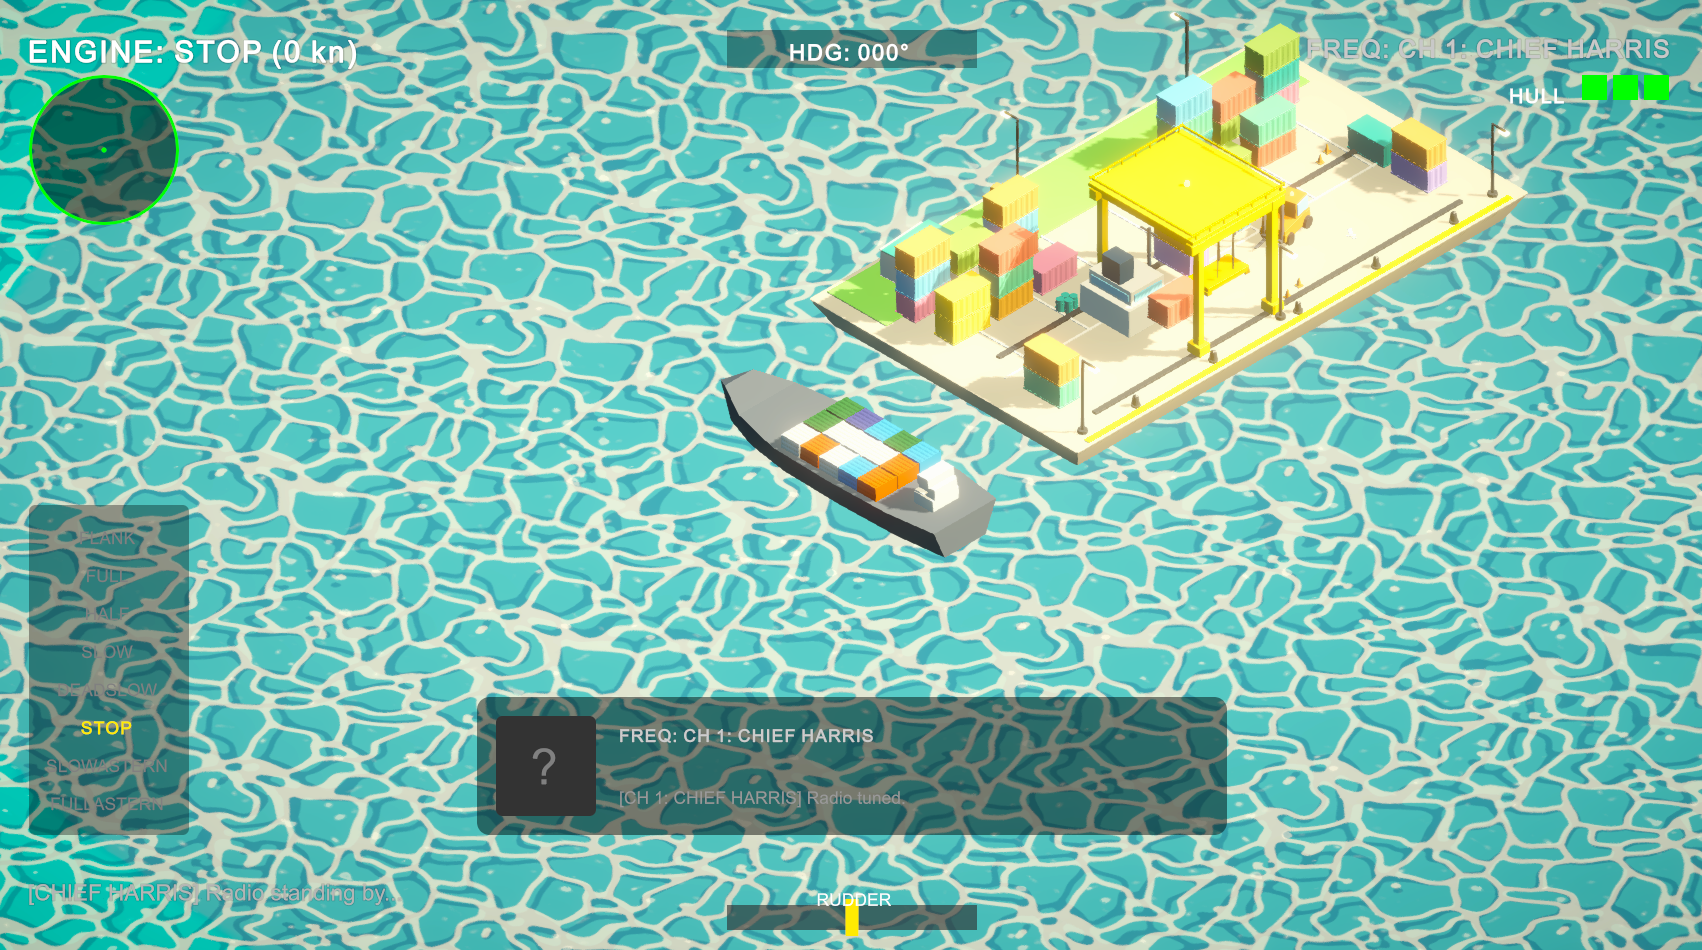
\includegraphics[width=\linewidth]{Document/GameDev/images/StartUI.png}\vspace{0.1cm} & 
\textbf{ฉากที่ 1: การรับมอบหมายภารกิจ}\newline
ผู้เล่นเริ่มต้นเกมในฐานะกัปตันเรือ หน้าจอแสดงบรรยากาศห้องบังคับการเรือ (Ship Bridge) พร้อมเสียงคลื่นและลมทะเล (Ambient Audio) เพื่อสร้างความรู้สึกดื่มด่ำ (Immersion) กัปตันได้รับมอบหมายให้นำเรือเดินทางไปยังจุดหมายปลายทางอย่างปลอดภัย \\ \hline

\vspace{0.1cm}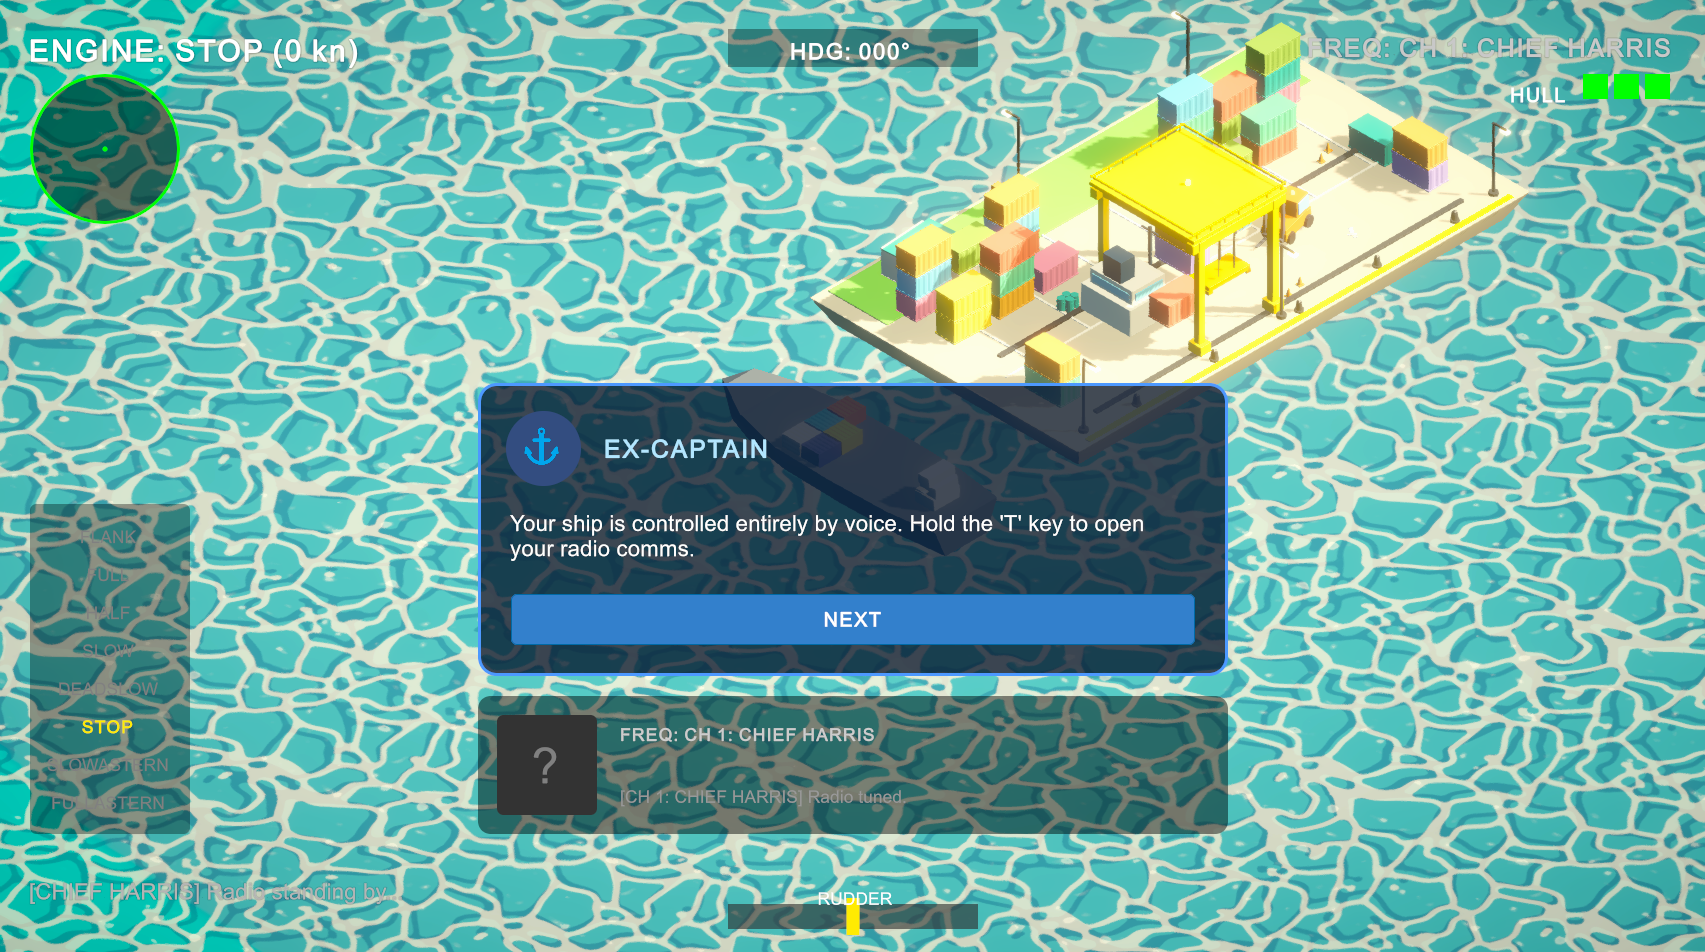
\includegraphics[width=\linewidth]{Document/GameDev/images/Tutorial.png}\vspace{0.1cm} &
\textbf{ฉากที่ 2: การแนะนำลูกเรือปัญญาประดิษฐ์}\newline
แนะนำตัวละครลูกเรือ AI สองตำแหน่ง ได้แก่ พลต้นหนผู้คอยแจ้งเตือนภัยจากเรดาร์ และพลถือท้ายผู้รอรับคำสั่งพวงมาลัย เกมเริ่มเข้าสู่โหมดการฝึกสอน (Tutorial) การออกคำสั่งเสียงภาษาอังกฤษพื้นฐาน \\ \hline

\vspace{0.1cm}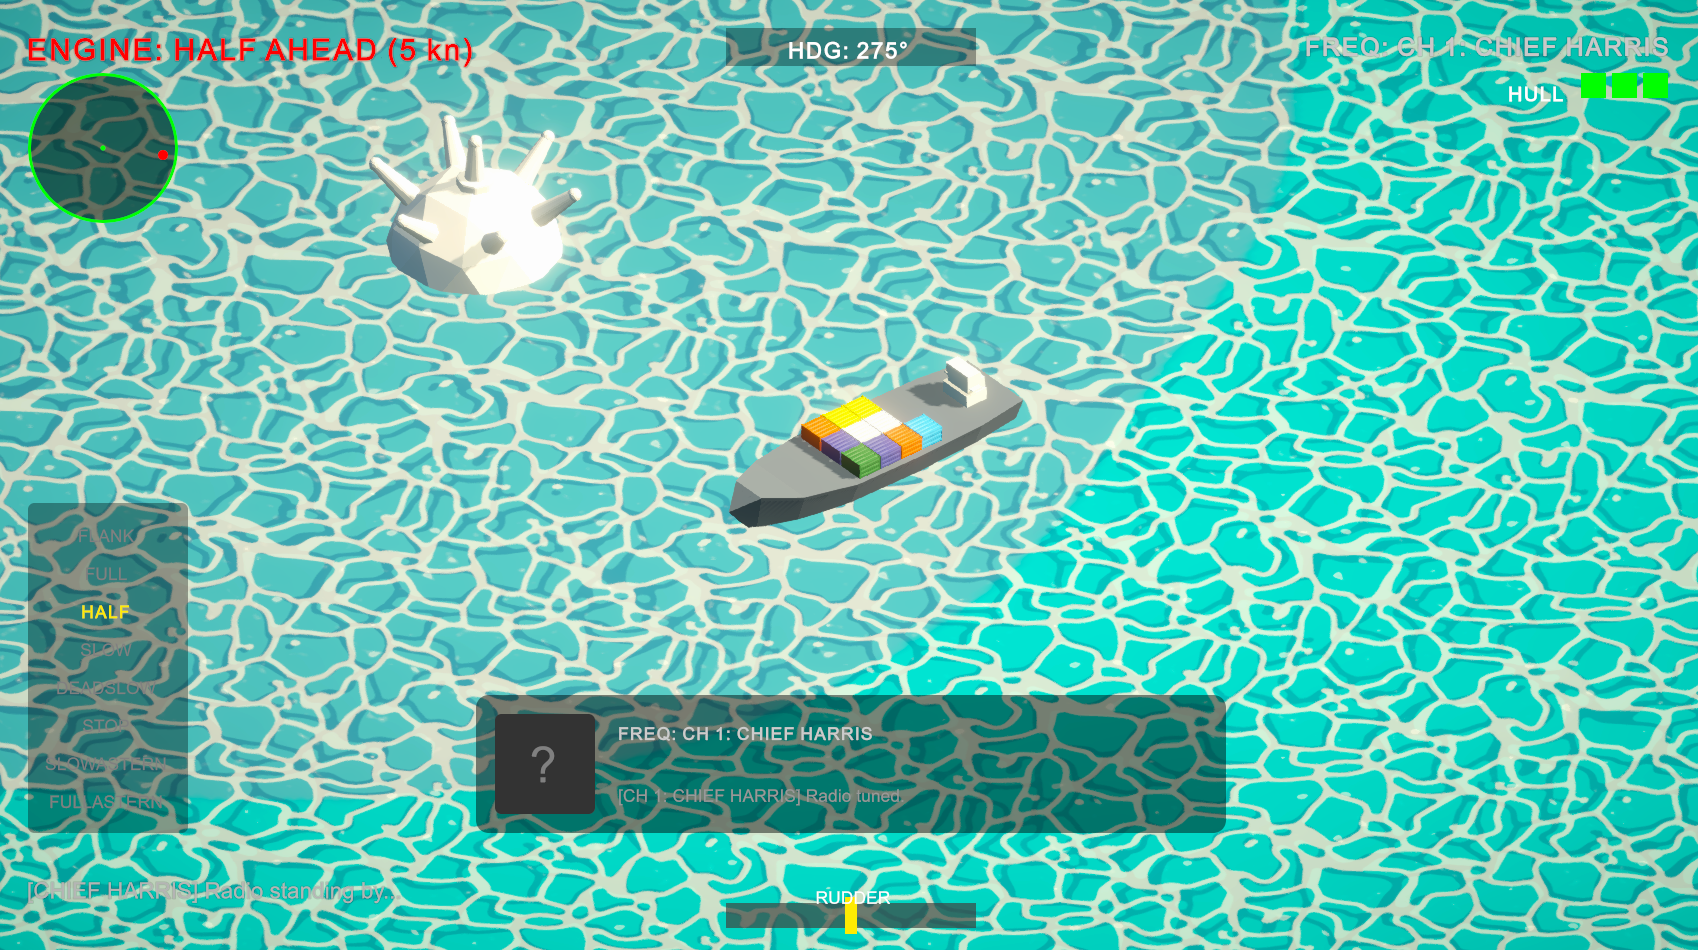
\includegraphics[width=\linewidth]{Document/GameDev/images/Hazard.png}\vspace{0.1cm} &
\textbf{ฉากที่ 3: สถานการณ์เผชิญหน้าสิ่งกีดขวาง}\newline
ระบบสุ่มสร้างอุปสรรค เช่น โขดหินหรือเรือลำอื่นขวางหน้า เรดาร์ส่งสัญญาณเตือนภัย ผู้เล่นต้องรีบประเมินสถานการณ์และเปล่งเสียงสั่งการแบบฉุกเฉินภายในเวลาที่กำหนด \\ \hline

\vspace{0.1cm}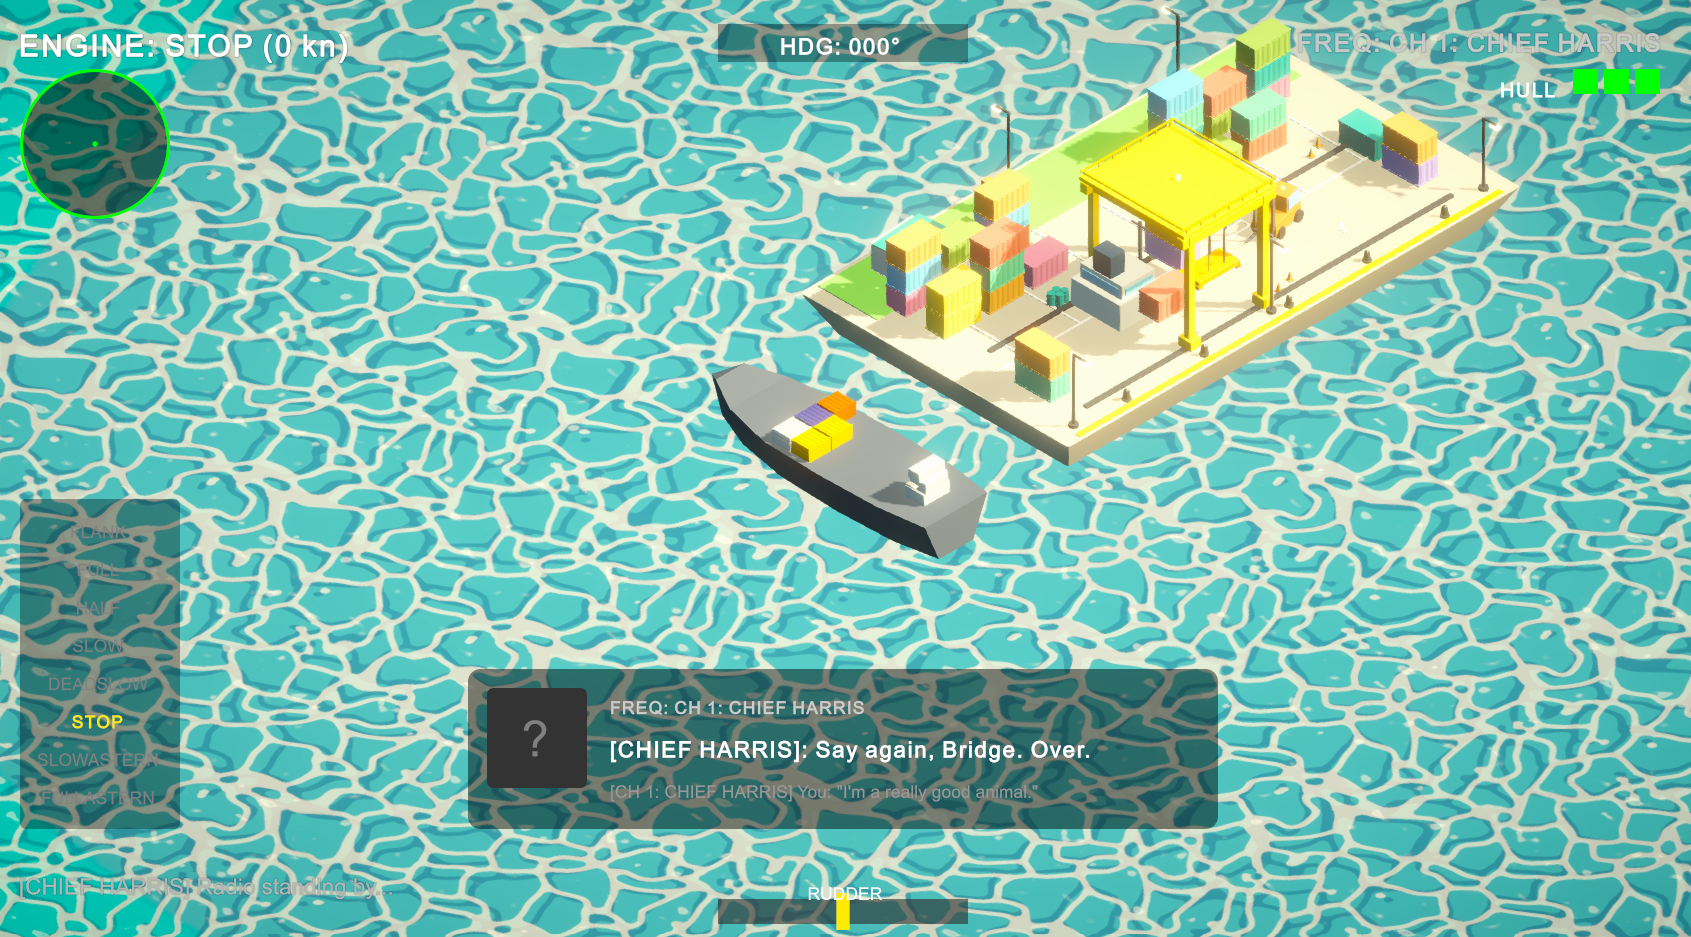
\includegraphics[width=\linewidth]{Document/GameDev/images/Sayagain.png}\vspace{0.1cm} & 
\textbf{ฉากที่ 4: สถานการณ์สื่อสารติดขัด (Clarification Request)}\newline
หากผู้เล่นออกเสียงไม่ชัดเจนหรือใช้คำสั่งผิดพลาด ลูกเรือ AI จะจำลองสถานการณ์สื่อสารติดขัดและทวนถาม เช่น \textit{``Say again, Captain?''} เพื่อกระตุ้นให้ผู้เล่นฝึกการแก้ปัญหาและเปล่งเสียงให้ชัดเจนขึ้น \\ \hline

\vspace{0.1cm}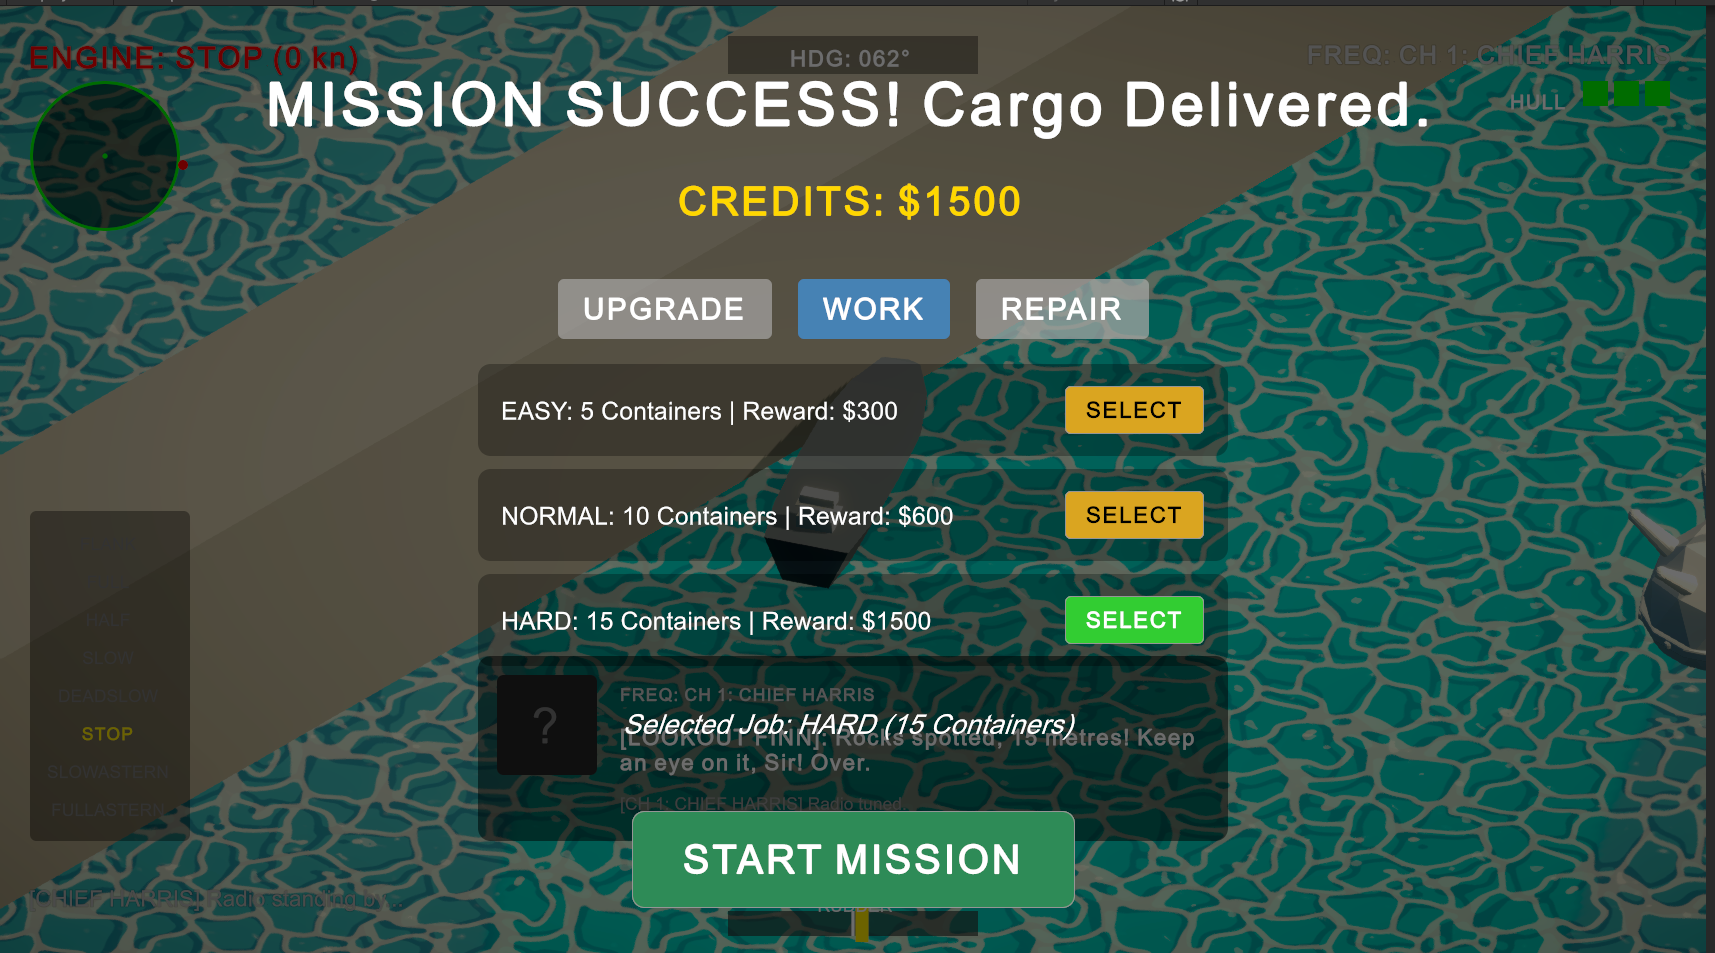
\includegraphics[width=\linewidth]{Document/GameDev/images/Victory.png}\vspace{0.1cm} & 
\textbf{ฉากที่ 5: สรุปผลภารกิจ (Result Screen)}\newline
หากนำเรือถึงเป้าหมายสำเร็จจะแสดงหน้าจอ Victory พร้อมสรุปคะแนนความแม่นยำในการออกเสียง แต่หากชนสิ่งกีดขวางจนมาตรวัดความเสียหายหมดลง จะแสดงหน้าจอ Game Over และต้องเริ่มภารกิจใหม่ \\
\hline
\end{tabular}
\end{table}
% -----------------------------------------------------------
\section{การออกแบบระบบการเล่น}
% -----------------------------------------------------------

\subsection{วิธีการเล่นเกม (How to Play)}

ในการเล่นเกมนี้ ผู้เล่นจะได้รับบทเป็นกัปตันเรือขนส่งสินค้า โดยมีหน้าที่ในการสั่งการลูกเรือเพื่อนำพาเรือเดินทางไปยังจุดหมายปลายทางอย่างปลอดภัย โดยกติกาการเล่นหลักมีดังนี้

\begin{enumerate}[label=\arabic*)]
    \item \textbf{เริ่มต้นภารกิจ:} ผู้เล่นเริ่มเกมด้วยการรับทราบเส้นทางเดินเรือและสภาพแวดล้อมเบื้องต้น
    \item \textbf{การควบคุมผ่านเสียง:} ผู้เล่นไม่สามารถใช้คีย์บอร์ดหรือเมาส์บังคับพวงมาลัยเรือโดยตรง แต่ต้องใช้ \textbf{คำสั่งเสียงภาษาอังกฤษ} (Voice Commands) สื่อสารกับลูกเรือ AI (พลต้นหน และ พลถือท้าย)
    \item \textbf{การหลบหลีกสิ่งกีดขวาง:} เมื่อเกมสุ่มสร้างสิ่งกีดขวาง (Obstacles) เช่น โขดหิน เกาะ หรือเรือลำอื่น ผู้เล่นต้องวิเคราะห์สถานการณ์จากมุมมองไอโซเมตริกและหน้าจอเรดาร์ จากนั้นออกคำสั่งที่เหมาะสม (เช่น "Starboard 15", "Stop Engine") ให้ทันเวลา
    \item \textbf{การตอบสนองของลูกเรือ:} 
    \begin{itemize}
        \item หากคำสั่งถูกต้องและชัดเจน พลถือท้ายจะบังคับเรือตามหลักฟิสิกส์ (มีแรงเฉื่อยและรัศมีวงเลี้ยว)
        \item หากคำสั่งไม่ถูกต้อง ผิดบริบท หรือออกเสียงไม่ชัดเจน ลูกเรือ AI จะทวนคำสั่งหรือขอให้ย้ำคำสั่ง (Clarification Request) ทำให้ผู้เล่นต้องเปล่งเสียงใหม่
    \end{itemize}
    \item \textbf{ผลลัพธ์ของภารกิจ:} 
    \begin{itemize}
        \item \textbf{สำเร็จ (Victory):} หากนำเรือถึงจุดหมายโดยหลบหลีกสิ่งกีดขวางได้ทั้งหมด
        \item \textbf{ล้มเหลว (Game Over):} หากชนสิ่งกีดขวางจนมาตรวัดความเสียหาย (Hull Integrity) ลดลงเหลือศูนย์
    \end{itemize}
\end{enumerate}

\subsection{กระบวนการเล่นหลัก (Core Game Loop)}

กระบวนการทำงานหลักของการเล่นเกม (Core Game Loop) ซึ่งสะท้อนการโต้ตอบระหว่างผู้เล่น, AI, และระบบฟิสิกส์ แสดงดังภาพที่ \ref{fig:gameloop}

\begin{figure}[H]
\centering
\begin{mermaid}
graph TD
    A[เริ่มภารกิจ] --> B[ประเมินสถานการณ์จากเรดาร์/สภาพแวดล้อม]
    B --> C{พบสิ่งกีดขวางหรือไม่?}
    C -- ไม่พบ --> D[รักษาเส้นทางและระดับความเร็ว]
    D --> B
    C -- พบสิ่งกีดขวาง --> E[ผู้เล่นออกคำสั่งเสียงภาษาอังกฤษฉุกเฉิน]
    E --> F[ระบบแปลงเสียงเป็นข้อความ Speech-to-Text]
    F --> G{คำสั่งชัดเจนและถูกต้องหรือไม่?}
    G -- ไม่ถูกต้อง/ไม่ชัดเจน --> H[ลูกเรือ AI จำลองการสื่อสารติดขัด และขอให้ย้ำคำสั่ง]
    H --> E
    G -- ถูกต้อง --> I[ลูกเรือ AI รับคำสั่งและตอบกลับ]
    I --> J[ระบบฟิสิกส์ควบคุมเรือเคลื่อนที่ตามคำสั่ง]
    J --> K{หลบหลีกสำเร็จหรือไม่?}
    K -- สำเร็จ --> L{ถึงจุดหมายหรือยัง?}
    L -- ยังไม่ถึง --> B
    L -- ถึงแล้ว --> M[ภารกิจสำเร็จ Victory]
    K -- ไม่สำเร็จ ชนสิ่งกีดขวาง --> N[มาตรวัดความเสียหาย Hull Integrity ลดลง]
    N --> O{ความเสียหายเหลือ 0 หรือไม่?}
    O -- ยังไม่เหลือ 0 --> B
    O -- เหลือ 0 --> P[ภารกิจล้มเหลว Game Over]
\end{mermaid}
\caption{แผนภาพกระบวนการเล่นหลัก (Core Game Loop)}
\label{fig:gameloop}
\end{figure}

จากภาพที่ \ref{fig:gameloop} แสดงให้เห็นว่าความท้าทายหลักของเกมไม่ได้อยู่ที่การบังคับปุ่ม แต่เป็นการบริหารเวลาในการ "เปล่งเสียง" และ "แก้ปัญหาการสื่อสาร" ภายใต้สถานการณ์ที่ระบบฟิสิกส์ของเรือยังคงดำเนินไปอย่างต่อเนื่อง

\subsection{การออกแบบส่วนติดต่อผู้ใช้ (UI/HUD Design)}

การออกแบบหน้าจอส่วนติดต่อผู้ใช้ (UI/HUD) ถูกออกแบบภายใต้แนวคิดการจำลองสถานการณ์ (Simulation Game Design) เพื่อให้ข้อมูลที่จำเป็นครบถ้วนแต่ไม่บดบังทัศนวิสัยหลัก รายละเอียดของส่วนประกอบบนหน้าจอ แสดงดังตารางที่ \ref{tab:hud}

\begin{table}[H]
\centering
\caption{องค์ประกอบของหน้าจอส่วนติดต่อผู้ใช้ (HUD)}
\label{tab:hud}
\begin{tabular}{|p{4.5cm}|p{9.2cm}|}
\hline
\textbf{องค์ประกอบหน้าจอ} & \textbf{บทบาทและหน้าที่} \\
\hline
มาตรวัดการเดินเรือ (Navigation Instruments) & แสดงเข็มทิศบอกองศาทิศทาง (Compass) และตัวแสดงองศาของพวงมาลัยหางเสือ (Rudder Angle Indicator) เพื่อให้กัปตันประเมินทิศทาง \\ \hline
สถานะเครื่องยนต์ (Engine Telegraph) & แสดงระดับความเร็วของเรือในปัจจุบัน \\ \hline
หน้าจอเรดาร์ (Radar Screen) & แสดงจุดของสิ่งกีดขวาง (Blips) รอบตัวเรือ เพื่อช่วยประเมินสถานการณ์ล่วงหน้า \\ \hline
สถานะการรับเสียง (Voice Input Indicator) & สัญลักษณ์รูปไมโครโฟนเพื่อแจ้งผู้เล่นว่าขณะนี้ระบบกำลังรับฟังเสียง หรือกำลังประมวลผลคำสั่ง \\ \hline
มาตรวัดความเสียหาย (Hull Integrity) & แถบพลังชีวิต (Health Bar) ของเรือ หากเกิดการชนแถบนี้จะลดลง \\
\hline
\end{tabular}
\end{table}

\pagebreak
\subsection{สถาปัตยกรรมของระบบ (System Architecture)}

สถาปัตยกรรมระบบเกมเดินเรือด้วยระบบสั่งการด้วยเสียงแสดงดังภาพที่ \ref{fig:architecture}

\begin{figure}[H]
\centering
\begin{mermaid}
graph TD
    subgraph Client["ส่วนของผู้เล่น (Client)"]
        Unity["Unity 3D Engine (Game Client)"]
        Mic["Microphone (Audio Input)"]
        Speaker["Speaker/Headphones (Audio Output)"]
    end

    subgraph Core["ส่วนประมวลผลหลัก (Core Systems)"]
        GameLogic["C# Game Logic & Ship Physics"]
        UI["UI & HUD Manager"]
    end

    subgraph ExternalAPI["ส่วนเชื่อมต่อภายนอก (External APIs)"]
        STT["Speech-to-Text API (Whisper)"]
        LLM["OpenAI API (GPT-4o mini)"]
    end

    Mic -->|Voice Input| Unity
    Unity -->|Audio Stream| STT
    STT -->|Text| GameLogic
    GameLogic -->|Text Prompt| LLM
    LLM -->|Voice/Text Feedback| GameLogic
    GameLogic -->|Control| UI
    GameLogic -->|Audio Feedback| Speaker
\end{mermaid}
\caption{สถาปัตยกรรมของระบบเกม}
\label{fig:architecture}
\end{figure}

จากภาพที่ \ref{fig:architecture} ระบบทำงานบน Game Engine Unity 3D เป็นหลัก โดยรับเสียงพูดภาษาอังกฤษผ่านไมโครโฟน ส่งไปแปลงเป็นข้อความด้วยเทคโนโลยีการรู้จำเสียง (Whisper API)\cite{aguirre2023} จากนั้นนำข้อความไปประมวลผลคำสั่งร่วมกับระบบฟิสิกส์เรือ หรือส่งต่อให้ปัญญาประดิษฐ์ (OpenAI GPT-4o mini) เพื่อสร้างบทสนทนาโต้ตอบจากลูกเรือ AI

\subsection{โครงสร้างโฟลเดอร์ของโครงการ (Project Structure)}

โครงสร้างแฟ้มข้อมูลของการพัฒนาโครงการบน Unity 3D แสดงดังตารางที่ \ref{tab:folder}

\begin{table}[H]
\centering
\caption{โครงสร้างโฟลเดอร์หลักของโครงการ}
\label{tab:folder}
\begin{tabular}{|p{4.5cm}|p{9.2cm}|}
\hline
\textbf{โฟลเดอร์} & \textbf{คำอธิบาย} \\
\hline
\texttt{Assets/Scenes/} & ฉากต่าง ๆ ภายในเกม (MainMenu, Gameplay, Shipyard, Result) \\ \hline
\texttt{Assets/Scripts/} & ชุดคำสั่งภาษา C\# สำหรับควบคุมระบบฟิสิกส์เรือ การรับคำสั่งเสียง และระบบ UI \\ \hline
\texttt{Assets/Scripts/API/} & ชุดคำสั่งสำหรับเชื่อมต่อ Speech-to-Text (Whisper) และ OpenAI API \\ \hline
\texttt{Assets/Prefabs/} & วัตถุสำเร็จรูป เช่น ตัวเรือ สิ่งกีดขวางที่ใช้ในการสุ่ม (Obstacle Generation) \\ \hline
\texttt{Assets/Models/} & แฟ้มโมเดล 3 มิติ (3D Models) ของเรือ สิ่งแวดล้อม และสิ่งกีดขวาง \\ \hline
\texttt{Assets/Audio/} & แฟ้มเสียงสภาพแวดล้อม (Ambient Audio) และเสียงเอฟเฟกต์ (SFX) สัญญาณเตือน \\ \hline
\texttt{Assets/UI/} & รูปภาพและกราฟิกสำหรับหน้าจอเรดาร์ เข็มทิศ และอินเทอร์เฟซผู้ใช้ \\
\hline
\end{tabular}
\end{table}

\subsection{การออกแบบหน้าจอ (UI Mockups)}

ต้นแบบหน้าจอ (Mockups) สำหรับเกมถูกออกแบบเพื่อจำลองสถานการณ์การเดินเรือ (Simulation) ให้ดูสมจริงและอ่านข้อมูลง่าย โดยมีหน้าจอหลักดังตารางที่ \ref{tab:mockups}

\begin{table}[H]
\centering
\caption{รายการต้นแบบหน้าจอ}
\label{tab:mockups}
\begin{tabular}{|p{1.5cm}|p{3.5cm}|p{8.5cm}|}
\hline
\textbf{รหัสหน้าจอ} & \textbf{ชื่อหน้าจอ} & \textbf{ส่วนประกอบหลัก} \\
\hline
UI-01 & หน้าจอหลัก (Main Menu) & ชื่อเกม, ปุ่มเริ่มเกม (Start Game), ปุ่มตั้งค่าระบบเสียง, ปุ่มออกเกม (Exit) \\ \hline
UI-02 & หน้าจอเล่นเกม (Gameplay HUD) & มุมมองไอโซเมตริกของเรือ, เข็มทิศ, หน้าจอเรดาร์, สถานะความเร็ว, สถานะไมโครโฟน, แถบความเสียหายเรือ \\ \hline
UI-03 & หน้าจออู่ต่อเรือ (Shipyard) & เมนูศูนย์กลางสำหรับนำเงินรางวัลมาซ่อมแซมหรืออัปเกรดประสิทธิภาพเรือ \\ \hline
UI-04 & หน้าจอสรุปผล (Result Screen) & หน้าจอแสดงผลเมื่อถึงเป้าหมายหรือเมื่อเรืออับปาง สรุปคะแนนความแม่นยำในการออกเสียง ความรวดเร็วในการสั่งการ \\
\hline
\end{tabular}
\end{table}

\subsubsection{UI-02: หน้าจอเล่นเกม (Gameplay HUD)}

หน้าจอส่วนติดต่อผู้ใช้ขณะเล่นเกมเป็นหน้าจอหลักที่ผู้เล่นจะต้องใช้งานตลอดการทำภารกิจ ออกแบบตามมุมมองไอโซเมตริก (Isometric View) แสดงภาพจำลองการจัดวางดังภาพที่ \ref{fig:wf_gameplay}

\begin{figure}[H]
\centering
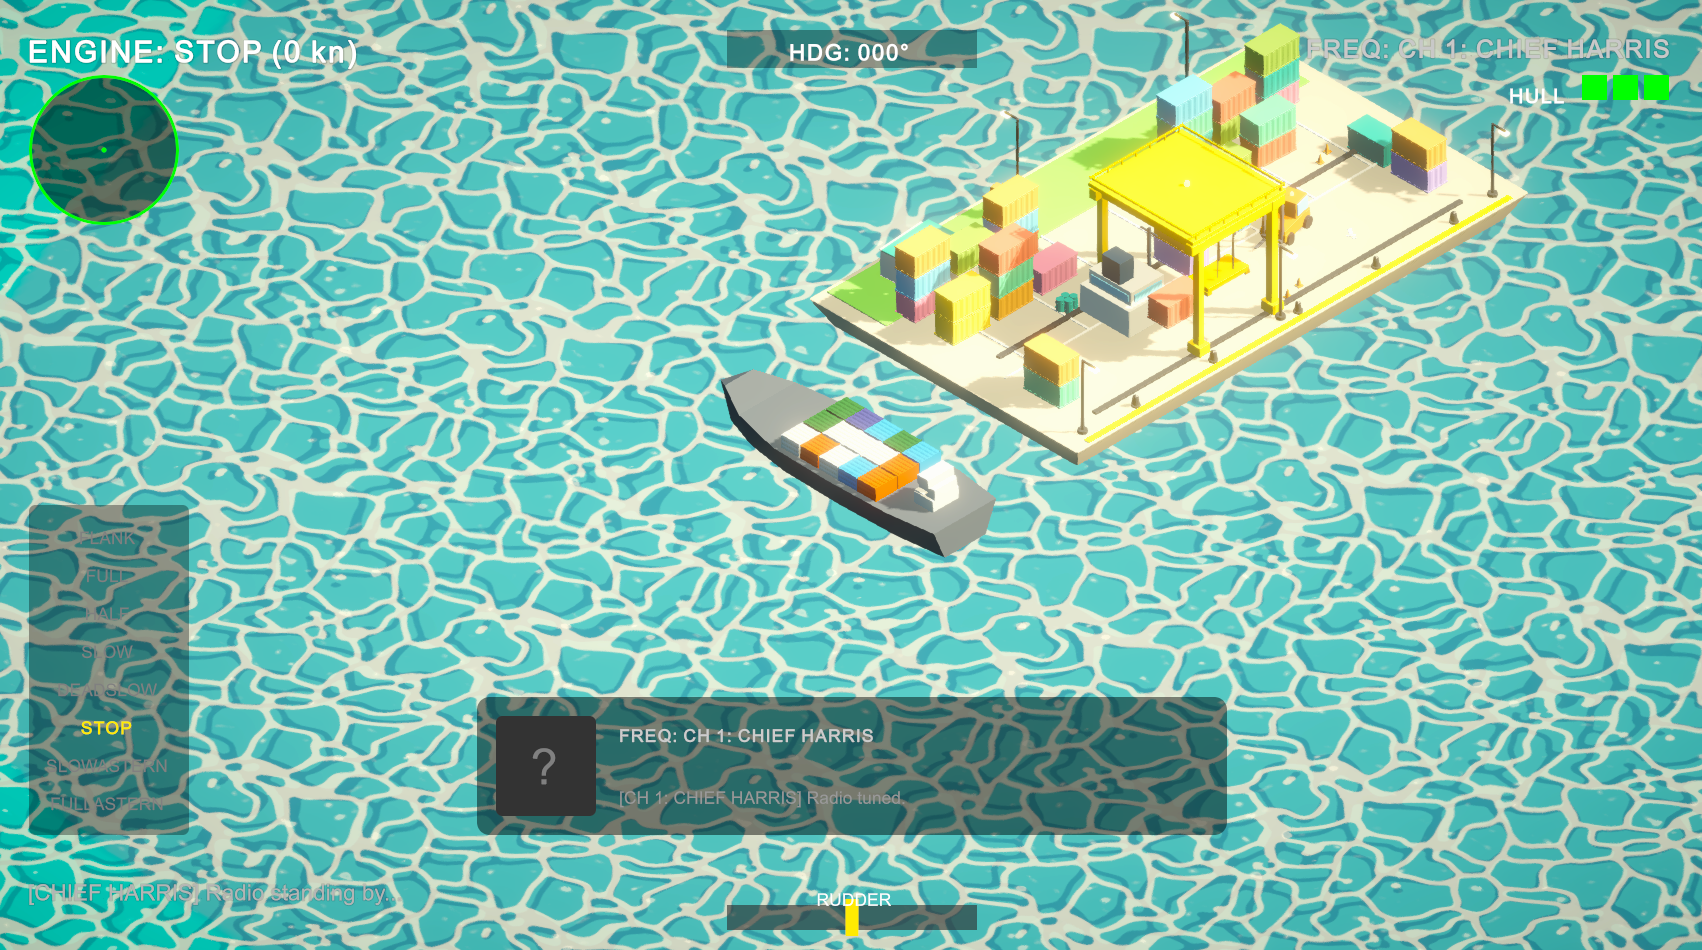
\includegraphics[width=0.8\textwidth]{Document/GameDev/images/StartUI.png}
\caption{ต้นแบบหน้าจอเล่นเกม (UI-02)}
\label{fig:wf_gameplay}
\end{figure}

จากภาพที่ \ref{fig:wf_gameplay} ผู้เล่นจะมองเห็นเรือจากมุมมองไอโซเมตริก เพื่อให้เห็นตัวเรือ สภาพแวดล้อมทางทะเล และตำแหน่งของสิ่งกีดขวางโดยรอบได้อย่างชัดเจน มุมหน้าจอจะมีมาตรวัดการเดินเรือ ได้แก่ เรดาร์ เข็มทิศบอกองศาทิศทาง และมาตรวัดความเร็ว นอกจากนี้ ด้านล่างจะมีสัญลักษณ์ไมโครโฟน (Voice Input Indicator) เพื่อแสดงสถานะว่าระบบกำลังรับฟัง หรือกำลังประมวลผลคำสั่ง เพื่อให้ผู้เล่นสามารถจับจังหวะการพูดและบริหารเวลาในการสื่อสารได้อย่างถูกต้อง
% =============================================================
% 4.3 การออกแบบองค์ประกอบในเกม
% โครงงาน: การออกแบบและพัฒนาเกมเดินเรือด้วยระบบสั่งการด้วยเสียงเพื่อส่งเสริมทักษะการสื่อสาร
% =============================================================

\section{การออกแบบองค์ประกอบในเกม}

องค์ประกอบภายในเกมได้รับการออกแบบเพื่อสร้างสภาพแวดล้อมจำลองที่สมจริง (Immersive Environment) และเอื้อต่อการเรียนรู้และการฝึกทักษะการสื่อสารภาษาอังกฤษ โดยแบ่งองค์ประกอบออกเป็น 3 ส่วนหลัก ดังนี้

\subsection{การออกแบบตัวละครและบทบาท (Characters and Roles)}

เกมจำลองสถานการณ์การทำงานร่วมกันบนห้องบังคับการเรือ โดยแบ่งบทบาทตัวละครออกเป็น 3 ตำแหน่งหลัก ดังนี้

\begin{enumerate}[label=\arabic*)]
    \item \textbf{กัปตัน (Captain):} ตัวแทนของผู้เล่น (Player Character) เป็นผู้มีอำนาจตัดสินใจสูงสุดและเป็นผู้ออกคำสั่งเสียงภาษาอังกฤษเพียงผู้เดียว
    \item \textbf{พลต้นหน (Navigator - AI):} ลูกเรือปัญญาประดิษฐ์ ทำหน้าที่ให้ข้อมูลด้านเส้นทาง เตือนภัยจากเรดาร์ และประเมินระยะห่างของสิ่งกีดขวาง เพื่อให้กัปตันนำข้อมูลไปตัดสินใจ
    \item \textbf{พลถือท้าย (Helmsman - AI):} ลูกเรือปัญญาประดิษฐ์ ทำหน้าที่รับคำสั่งจากกัปตันโดยตรงเพื่อบังคับพวงมาลัยหางเสือและคันเร่งเครื่องยนต์ พร้อมทั้งให้เสียงทวนคำสั่ง (Voice Feedback) เพื่อยืนยันความเข้าใจ
\end{enumerate}

\subsection{การออกแบบอุปสรรคและสิ่งกีดขวาง (Obstacles and Hazards)}

เพื่อให้เกมมีความท้าทายและป้องกันไม่ให้ผู้เล่นใช้การท่องจำเส้นทาง (Memorization) ระบบจึงใช้การสุ่มสร้างสิ่งกีดขวาง (Obstacle Generation System) รูปแบบของอุปสรรคที่ออกแบบไว้ ได้แก่

\begin{itemize}
    \item \textbf{สิ่งกีดขวางทางธรรมชาติ:} เช่น โขดหินใต้น้ำ เกาะ หรือภูเขาน้ำแข็ง ที่บีบบังคับให้ผู้เล่นต้องประเมินระยะห่างและสั่งการเลี้ยวหลบให้ทันเวลา
    \item \textbf{สิ่งกีดขวางแบบเคลื่อนที่:} เช่น เรือลำอื่นที่สัญจรไปมาในช่องแคบที่พลุกพล่าน ทำให้ผู้เล่นต้องฝึกไหวพริบและแก้ไขสถานการณ์เฉพาะหน้า
\end{itemize}

\subsection{การออกแบบกราฟิกและเสียงประกอบ (Graphic \& Audio Design)}

การออกแบบด้านทัศนศิลป์และเสียงมุ่งเน้นไปที่การสร้างความรู้สึกดื่มด่ำ (Immersion) ให้ผู้เล่นรู้สึกเหมือนกำลังบัญชาการเรือจริง ๆ

\begin{itemize}
    \item \textbf{กราฟิก (Graphic):} นำเสนอในมุมมองการเล่นแบบไอโซเมตริก (Isometric View) เพื่อให้ผู้เล่นสามารถมองเห็นตัวเรือ สภาพแวดล้อมทางทะเล และตำแหน่งของสิ่งกีดขวางโดยรอบได้อย่างชัดเจนในมุมกว้าง
    \item \textbf{เสียงแวดล้อม (Ambient Audio):} มีการใส่เสียงคลื่น เสียงลมทะเล และเสียงการทำงานของเครื่องยนต์เรืออย่างต่อเนื่อง เพื่อสร้างบรรยากาศการเดินเรือที่สมจริง
    \item \textbf{เสียงเอฟเฟกต์ (SFX):} ใช้เสียงสัญญาณเตือนภัย (Alarm) จากเรดาร์เมื่อเรือเคลื่อนเข้าใกล้สิ่งกีดขวาง เพื่อกระตุ้นความตื่นตัวและสร้างความกดดันด้านเวลาให้ผู้เล่นต้องรีบออกคำสั่ง
\end{itemize}
% =============================================================
% 4.4 การออกแบบเชิงการศึกษาและการประเมินผล
% โครงงาน: การออกแบบและพัฒนาเกมเดินเรือด้วยระบบสั่งการด้วยเสียงเพื่อส่งเสริมทักษะการสื่อสาร
% =============================================================

\section{การออกแบบเชิงการศึกษาและการประเมินผล}

เนื่องจากโครงงานนี้เป็นเกมเพื่อการเรียนรู้แบบจริงจัง (Serious Game) การออกแบบจึงบูรณาการกลไกของเกม (Gamification) เข้ากับทฤษฎีการเรียนรู้ภาษา เพื่อให้ผู้เล่นได้รับการพัฒนาทักษะเชิงปฏิบัติอย่างมีประสิทธิภาพ\cite{sadigzade2025} โดยแบ่งออกเป็น 2 ส่วน ดังนี้

\subsection{การออกแบบเชิงการศึกษา (Educational Design)}

การออกแบบกลไกเพื่อส่งเสริมการเรียนรู้ประกอบด้วยแนวคิดหลัก ดังนี้

\begin{enumerate}[label=\arabic*)]
    \item \textbf{การเรียนรู้ตามสถานการณ์ (Situated Learning):} ผู้เล่นจะไม่ได้เรียนรู้คำศัพท์จากการท่องจำ แต่จะได้เรียนรู้ผ่านการจำลองสถานการณ์เดินเรือจริง (Maritime Communication) เช่น การสั่งหันหางเสือหรือการปรับความเร็ว เพื่อให้เกิดความเข้าใจในบริบทและสามารถนำไปประยุกต์ใช้ได้ทันที\cite{sadigzade2025}
    \item \textbf{การลดตัวกรองทางอารมณ์ (Affective Filter Hypothesis):} การให้ผู้เล่นฝึกเปล่งเสียงสั่งการกับ "ลูกเรือปัญญาประดิษฐ์ (AI Crew)" แทนการสนทนากับมนุษย์จริง จะช่วยสร้างพื้นที่ปลอดภัย (Safe Space) ลดความกลัวความผิดพลาด และบรรเทาความวิตกกังวลในการใช้ภาษาต่างประเทศ (Language Anxiety)\cite{sadigzade2025}
    \item \textbf{การเรียนรู้จากข้อผิดพลาด (Learning from Failure):} เมื่อผู้เล่นเปล่งเสียงไม่ชัดเจนหรือผิดหลักไวยากรณ์ ระบบจะไม่ลงโทษด้วยการตัดจบทันที แต่ลูกเรือ AI จะใช้กลไกการทวนถาม (Clarification Request) ซึ่งเป็นการให้ข้อมูลป้อนกลับ (Feedback) เพื่อกระตุ้นให้ผู้เล่นแก้ไขการพูดด้วยตนเอง\cite{zargham2024}
\end{enumerate}

\subsection{แนวทางการประเมินผล (Evaluation Approach)}

การประเมินผลของเกมถูกออกแบบให้ครอบคลุมทั้งประสิทธิภาพของเทคโนโลยีและผลสัมฤทธิ์ด้านการเรียนรู้ของผู้เล่น ดังนี้

\begin{itemize}
    \item \textbf{การประเมินผลภายในเกม (In-game Evaluation):} ประเมินจากความแม่นยำในการออกเสียงคำสั่ง (Speech Accuracy) ความรวดเร็วในการสั่งการแก้ไขปัญหาเฉพาะหน้า และสภาพความสมบูรณ์ของตัวเรือ (Hull Integrity) ที่เหลืออยู่เมื่อจบภารกิจ
    \item \textbf{การประเมินประสิทธิภาพทางเทคนิค (Technical Evaluation):} ประเมินอัตราความแม่นยำในการแปลคำสั่งเสียงของระบบ Speech-to-Text และวัดค่าความหน่วง (Latency) ของระบบตั้งแต่ผู้เล่นพูดจบจนถึงตอนที่เรือเริ่มตอบสนอง
    \item \textbf{การประเมินประสบการณ์ผู้เล่น (User Experience Evaluation):} ประเมินผ่านแบบสอบถามหลังการเล่นกับกลุ่มเป้าหมาย เพื่อวัดระดับความรู้สึกดื่มด่ำ (Immersion) รวมถึงความมั่นใจที่เพิ่มขึ้นและความวิตกกังวลที่ลดลงในการใช้ภาษาอังกฤษ
\end{itemize}
% =============================================================
% 4.5 การพัฒนาเกม
% โครงงาน: การออกแบบและพัฒนาเกมเดินเรือด้วยระบบสั่งการด้วยเสียงเพื่อส่งเสริมทักษะการสื่อสาร
% =============================================================

\section{การพัฒนาเกม}

การพัฒนาเกมดำเนินการบนเอนจิน Unity 3D และใช้ภาษา C\# เป็นหลัก โดยแบ่งการพัฒนาออกเป็นระบบย่อยและการบูรณาการเทคโนโลยีปัญญาประดิษฐ์เข้ากับกลไกของเกม ดังนี้

\subsection{การพัฒนาระบบรับคำสั่งเสียง (Speech Recognition System)}
ระบบรับคำสั่งเสียงถูกพัฒนาโดยการเชื่อมต่อไมโครโฟนเข้ากับ API หรือไลบรารีสำหรับการรู้จำเสียงอย่าง Whisper\cite{aguirre2023} เพื่อทำหน้าที่รับสัญญาณเสียงพูดภาษาอังกฤษของผู้เล่นแบบเรียลไทม์ และแปลงข้อมูลเสียงให้เป็นข้อความ (Speech-to-Text) จากนั้นจะส่งข้อความที่ได้เข้าสู่ระบบคัดกรองคำสั่ง (Text Parsing) เพื่อเตรียมนำไปประมวลผลบังคับเรือต่อไป

\begin{figure}[H]
\centering
\includegraphics[width=0.8\textwidth]{Document/GameDev/images/forth.png}
\caption{รหัสคำสั่งส่วนการรับคำสั่งเสียงและการแปลงเป็นข้อความ}
\label{fig:code_speech}
\end{figure}

\subsection{การพัฒนาระบบลูกเรือปัญญาประดิษฐ์ (AI Crew System)}
ระบบนี้ใช้บริการเชื่อมต่อ API ของ OpenAI (เช่น GPT-4o mini) เข้ามาช่วยในการตีความและโต้ตอบ เมื่อระบบได้รับข้อความคำสั่งจากผู้เล่น AI จะทำการตรวจสอบความถูกต้องของบริบทและไวยากรณ์ หากคำสั่งถูกต้อง AI จะส่งคำสั่งไปควบคุมตัวเรือ แต่หากคำสั่งไม่ชัดเจน AI จะทำการสร้างบทสนทนาโต้ตอบกลับ (Voice Feedback) เพื่อขอให้ผู้เล่นย้ำคำสั่ง

\begin{figure}[H]
\centering
\includegraphics[width=0.8\textwidth]{Document/GameDev/images/fifth.png}
\caption{รหัสคำสั่งส่วนการประมวลผลคำสั่งลูกเรือ AI และการโต้ตอบ}
\label{fig:code_ai_crew}
\end{figure}

\subsection{การพัฒนาระบบฟิสิกส์และการควบคุมเรือ (Ship Physics)}
การควบคุมเรือถูกเขียนด้วยภาษา C\# เพื่อจำลองการเคลื่อนที่ของเรือขนาดใหญ่ โดยมีการคำนวณตัวแปรด้านความเฉื่อย (Inertia) และรัศมีวงเลี้ยว (Turning Radius) ทำให้เรือไม่ตอบสนองต่อการเลี้ยวหรือการเบรกในทันทีที่ได้รับคำสั่ง 

\begin{figure}[H]
\centering
\includegraphics[width=0.8\textwidth]{Document/GameDev/images/sixth.png}
\caption{รหัสคำสั่งส่วนระบบฟิสิกส์และการจำลองการเดินเรือ}
\label{fig:code_physics}
\end{figure}

\subsection{ระยะการพัฒนาเกม (Development Phases)}
การดำเนินการพัฒนาเกมตัวต้นแบบถูกแบ่งออกเป็น 4 ระยะหลัก เพื่อให้การทำงานเป็นระบบและสามารถทดสอบได้ในแต่ละขั้นตอน ดังนี้

\begin{enumerate}[label=\arabic*)]
    \item \textbf{ระยะที่ 1 (Prototype):} พัฒนาระบบพื้นฐาน โดยเน้นการเชื่อมต่อระบบไมโครโฟนเข้ากับ Speech-to-Text API และทดสอบการแปลงเสียงเป็นข้อความคำสั่ง (Text Parsing) เพื่อขยับวัตถุเรือเบื้องต้น
    \item \textbf{ระยะที่ 2 (Alpha):} พัฒนาระบบสภาพแวดล้อมทางทะเล การสุ่มเกิดของสิ่งกีดขวาง (Obstacle Generation) และใส่ระบบเสียงโต้ตอบ (Voice-over) ของลูกเรือ AI
    \item \textbf{ระยะที่ 3 (Beta):} พัฒนาระบบ UI/UX ให้สมบูรณ์ ปรับจูนความยากง่าย (เช่น ความเร็วของเรือ ระยะห่างของสิ่งกีดขวาง) และความแม่นยำ (Tolerance) ในการรับคำสั่งเสียง
    \item \textbf{ระยะที่ 4 (Public/Release Candidate):} ตรวจสอบและแก้ไขข้อผิดพลาด (Bug Fixing) และเตรียมแพ็กเกจเกมสำหรับนำไปทดสอบกับผู้ใช้งานจริง
\end{enumerate}


\chapter{สรุปผลการดำเนินงาน}
% =============================================================
% บทที่ 5 - สรุปผลและอภิปรายผล
% โครงงาน: การออกแบบและพัฒนาเกมเดินเรือด้วยระบบสั่งการด้วยเสียงเพื่อส่งเสริมทักษะการสื่อสาร
% =============================================================

\section{สรุปผลการดำเนินงาน}

รายงานความก้าวหน้าฉบับนี้สรุปผลการดำเนินงานในระยะที่ 1 ของโครงงานการออกแบบและพัฒนาเกมเดินเรือด้วยระบบสั่งการด้วยเสียง (Voice-Controlled Ship Navigation Game) เพื่อส่งเสริมทักษะการสื่อสาร ซึ่งครอบคลุมการศึกษาทฤษฎีและงานวิจัยที่เกี่ยวข้อง การออกแบบระบบและกลไกการเล่น และการพัฒนาเกมต้นแบบ (Prototype) โดยผู้จัดทำได้ดำเนินการแล้วเสร็จในส่วนต่าง ๆ ดังนี้

ด้านการออกแบบ ผู้จัดทำได้ออกแบบเนื้อเรื่องและสตอรี่บอร์ด กระบวนการเล่นหลัก (Core Game Loop) สถาปัตยกรรมของระบบ ส่วนติดต่อผู้ใช้ (UI/HUD) และบทบาทของตัวละครทั้งสามตำแหน่ง ได้แก่ กัปตัน (ผู้เล่น) พลต้นหน และพลถือท้าย รวมถึงจัดทำคลังคำสั่งการเดินเรือมาตรฐาน (Standard Marine Communication Phrases) สำหรับใช้เป็นเกณฑ์ตรวจสอบความถูกต้องของคำสั่งเสียง ดังแสดงในภาคผนวก ง

ด้านการพัฒนา ได้พัฒนาเกมต้นแบบบนเอนจิน Unity 3D ด้วยภาษา C\# และเชื่อมต่อระบบย่อยหลักได้สำเร็จ 3 ระบบ ได้แก่ (1) ระบบรับคำสั่งเสียง ซึ่งรับสัญญาณจากไมโครโฟนและแปลงเป็นข้อความผ่าน Whisper API (2) ระบบลูกเรือปัญญาประดิษฐ์ ซึ่งส่งข้อความคำสั่งไปตีความผ่าน OpenAI API และสร้างบทสนทนาโต้ตอบกลับ และ (3) ระบบฟิสิกส์และการควบคุมเรือ ซึ่งจำลองความเฉื่อย (Inertia) และรัศมีวงเลี้ยว (Turning Radius) ของเรือขนาดใหญ่ ผลการทดสอบเบื้องต้นในระดับหน่วย (Unit Testing) พบว่าระบบสามารถรับคำสั่งเสียง แปลงเป็นข้อความ ส่งต่อไปยังตัวแยกคำสั่ง (Command Router) และควบคุมการเคลื่อนที่ของเรือได้อย่างต่อเนื่องตามที่ออกแบบไว้ รวมถึงสามารถจำลองสถานการณ์สื่อสารติดขัด (Communication Breakdown) โดยให้ลูกเรือ AI ทวนถามเมื่อคำสั่งไม่ชัดเจนได้ตามกลไกที่กำหนด

งานที่อยู่ระหว่างดำเนินการ ได้แก่ การพัฒนาระบบสุ่มสร้างสิ่งกีดขวาง (Obstacle Generation System) และระบบอินเทอร์เฟซผู้ใช้ (UI/HUD) ให้สมบูรณ์ การปรับจูนระดับความยากและค่าความคลาดเคลื่อนที่ยอมรับได้ (Tolerance) ของการรับคำสั่งเสียง ตลอดจนการทดสอบแบบบูรณาการ (Integration Testing) และการทดสอบการยอมรับของผู้ใช้ (User Acceptance Testing)

ในส่วนของการประเมินผล ยังไม่ได้ดำเนินการเก็บข้อมูลในระยะนี้ โดยผู้จัดทำมีแผนจะประเมินประสิทธิภาพทางเทคนิค (ความแม่นยำและความหน่วงของระบบ Speech-to-Text) และประเมินประสบการณ์ผู้ใช้ ความมั่นใจ และระดับความวิตกกังวลในการใช้ภาษาอังกฤษ กับกลุ่มตัวอย่างจำนวน 40–50 คน ในระยะถัดไป ซึ่งผลการประเมินดังกล่าวจะเป็นข้อมูลสำหรับสรุปว่าระบบบรรลุวัตถุประสงค์ในการลดความวิตกกังวลในการใช้ภาษาต่างประเทศ (Foreign Language Anxiety) ได้มากน้อยเพียงใด

\section{ปัญหาและข้อจำกัด}

ในการดำเนินโครงงานและพัฒนาตัวเกมต้นแบบ ผู้จัดทำพบปัญหาและข้อจำกัดที่ส่งผลต่อประสิทธิภาพของระบบและการประเมินผล ดังนี้

\begin{enumerate}[label=\arabic*)]
    \item \textbf{ข้อจำกัดด้านฮาร์ดแวร์และสภาพแวดล้อม:} ประสิทธิภาพและความแม่นยำในการรับคำสั่งของเกมขึ้นอยู่กับคุณภาพของไมโครโฟนที่ผู้เล่นใช้งาน รวมถึงหากสภาพแวดล้อมขณะเล่นมีเสียงรบกวนภายนอก (Background Noise) มากเกินไป จะส่งผลให้ระบบรับคำสั่งผิดพลาดได้ง่าย
    \item \textbf{ข้อจำกัดด้านระบบการรู้จำเสียง:} ระบบ Speech-to-Text มีข้อจำกัดในการทำความเข้าใจสำเนียง (Accent) ที่หลากหลายของผู้เล่นที่ไม่ใช่เจ้าของภาษา (Non-native speakers) 
    \item \textbf{ข้อจำกัดด้านขอบเขตการสื่อสาร:} โครงงานนี้ออกแบบมารองรับเฉพาะชุดคำสั่งภาษาอังกฤษเกี่ยวกับการเดินเรือที่กำหนดไว้ล่วงหน้าเท่านั้น ไม่รองรับการสนทนาโต้ตอบแบบอิสระ (Free-form Conversation)
    \item \textbf{ข้อจำกัดด้านกลุ่มตัวอย่างและการประเมินผล:} การประเมินผลอาศัยกลุ่มตัวอย่างจำนวนน้อย (40–50 คน) ภายในบริบทของมหาวิทยาลัย ซึ่งอาจไม่สะท้อนผลลัพธ์ของประชากรในวงกว้างทั้งหมดได้ และเกมเป็นเพียงเครื่องมือเสริม ไม่สามารถใช้ทดแทนการทดสอบมาตรฐานทางภาษาเชิงลึกได้
\end{enumerate}

\section{แนวทางการแก้ไขและข้อเสนอแนะ}

เพื่อให้การพัฒนาเกมมีความสมบูรณ์และสามารถนำไปต่อยอดได้ในอนาคต ผู้จัดทำมีแนวทางการแก้ไขและข้อเสนอแนะ ดังนี้

\begin{enumerate}[label=\arabic*)]
    \item \textbf{การจัดการเสียงรบกวน:} ผู้พัฒนาควรแนะนำให้ผู้เล่นใช้งานชุดหูฟังที่มีไมโครโฟนในตัว หรืออาจต้องศึกษาการพัฒนาระบบกรองเสียงรบกวนเบื้องต้น (Noise Filter) ก่อนส่งข้อมูลเสียงไปยัง API เพื่อเพิ่มความแม่นยำในการรับคำสั่ง
    \item \textbf{การปรับปรุงความแม่นยำในการรับคำสั่ง:} ควรมีการรวบรวมข้อมูล หรือปรับค่าความคลาดเคลื่อน (Tolerance) ของคำสั่งที่อนุโลมได้ เพื่อรองรับสำเนียงที่หลากหลายและลดความหงุดหงิดของผู้เล่น
    \item \textbf{การขยายขอบเขตในอนาคต:} ในอนาคตสามารถขยายระบบคลังคำศัพท์ (Command Vocabulary) ให้รองรับรูปแบบการสื่อสารทางทะเลที่ซับซ้อนยิ่งขึ้น และเพิ่มการประเมินผลกับกลุ่มตัวอย่างที่ใหญ่ขึ้น เพื่อประเมินผลสัมฤทธิ์ด้านการลดตัวกรองทางอารมณ์ (Affective Filter) ในระดับที่ครอบคลุมกว่าเดิม
\end{enumerate}

% ==========================================
% เอกสารอ้างอิง
% ==========================================
\clearpage
\addcontentsline{toc}{chapter}{เอกสารอ้างอิง}
\makeatletter
\let\ps@plain\ps@empty
\makeatother
\nocite{*}
\bibliographystyle{ieeetr}
\bibliography{references}
% ==========================================
% ภาคผนวก
% ==========================================
% =============================
% ภาคผนวก 
% =============================

% =============================
% ภาคผนวก ก — แบบสอบถามความคิดเห็นผู้เล่น
% =============================
\setcounter{chapter}{-1}
\appendiceschapter{แบบสอบถามความคิดเห็นผู้เล่น}

\section*{แบบสอบถามความคิดเห็นผู้เล่น}

\textbf{คำชี้แจง} แบบสอบถามนี้จัดทำขึ้นเพื่อประเมินความคิดเห็นของผู้เล่นที่ได้ทดลองเล่นเกมเดินเรือด้วยระบบสั่งการด้วยเสียงเพื่อส่งเสริมทักษะการสื่อสาร โดยข้อมูลที่ได้รับจะนำไปใช้เพื่อปรับปรุงและพัฒนาต่อไป

\subsection*{ตอนที่ 1 ข้อมูลทั่วไป}
1. เพศ: $\square$ ชาย \quad $\square$ หญิง \quad $\square$ อื่น ๆ \newline
2. อายุ: \rule{2cm}{0.4pt} ปี \newline
3. ระดับการศึกษา: $\square$ ปริญญาตรี \quad $\square$ ปริญญาโท \quad $\square$ อื่น ๆ

\subsection*{ตอนที่ 2 ความคิดเห็นต่อเกม}
โปรดเลือกคำตอบที่ตรงกับความคิดเห็นของท่านมากที่สุด

\begin{table}[H]
\centering
\caption{แบบสอบถามความคิดเห็นต่อเกมเดินเรือด้วยระบบสั่งการด้วยเสียง}
\label{tab:survey_game}
\small
% ปรับขนาดคอลัมน์แรกจาก p{7.5cm} เป็น p{5cm} เพื่อไม่ให้ตารางล้นขอบ
\begin{tabular}{|p{5cm}|c|c|c|c|c|}
\hline
\textbf{ข้อคำถาม} & \textbf{เห็นด้วยมาก} & \textbf{เห็นด้วย} & \textbf{ปานกลาง} & \textbf{ไม่เห็นด้วย} & \textbf{ไม่เห็นด้วยเลย} \\ \hline
1. เนื้อหาของเกมและรูปแบบการสั่งการด้วยเสียงเข้าใจง่าย & $\square$ & $\square$ & $\square$ & $\square$ & $\square$ \\ \hline
2. สภาพแวดล้อมจำลองและระบบฟิสิกส์การเดินเรือมีความสมจริง & $\square$ & $\square$ & $\square$ & $\square$ & $\square$ \\ \hline
3. การโต้ตอบและการทวนคำสั่งของลูกเรือ AI มีความน่าสนใจและสมจริง & $\square$ & $\square$ & $\square$ & $\square$ & $\square$ \\ \hline
4. เกมช่วยลดความวิตกกังวลและเพิ่มความมั่นใจในการพูดภาษาอังกฤษ & $\square$ & $\square$ & $\square$ & $\square$ & $\square$ \\ \hline
5. โดยรวมแล้วรู้สึกสนุกและมีแรงจูงใจในการฝึกฝนทักษะการสื่อสาร & $\square$ & $\square$ & $\square$ & $\square$ & $\square$ \\ \hline
\end{tabular}
\end{table}

\subsection*{ตอนที่ 3 ข้อเสนอแนะเพิ่มเติม}
\noindent\rule{\textwidth}{0.4pt}\\[0.5cm]
\noindent\rule{\textwidth}{0.4pt}\\[0.5cm]
\noindent\rule{\textwidth}{0.4pt}


% =============================
% ภาคผนวก ข — รหัสต้นฉบับ (Source Code)
% =============================
\appendiceschapter{รหัสต้นฉบับ}
\section*{ส่วนที่ 1: รหัสคำสั่งส่วนการเชื่อมต่อและรู้จำเสียง (Speech-to-Text)}
\textit{ส่วนนี้แสดงตัวอย่างโค้ด C\# สำหรับรับเสียงจากไมโครโฟนและแปลงเป็นข้อความ (Speech-to-Text) ผ่าน Whisper API}


\begin{figure}[H]
\centering
\includegraphics[width=0.8\textwidth]{Document/GameDev/images/seventh.png}
\caption{โค้ดสำหรับรับคำสั่งเสียงและแปลงเป็นข้อความ}
\label{fig:code_stt}
\end{figure}
\section*{ส่วนที่ 2: รหัสคำสั่งส่วนระบบฟิสิกส์ยานพาหนะ (Ship Navigation Physics)}
\textit{ส่วนนี้แสดงตัวอย่างโค้ด C\# ในการคำนวณแรงเฉื่อย (Inertia) และรัศมีวงเลี้ยวของเรือ}


\begin{figure}[H]
\centering
\includegraphics[width=0.8\textwidth]{Document/GameDev/images/eight.png}
\caption{โค้ดระบบจำลองฟิสิกส์การเคลื่อนที่ของเรือ}
\label{fig:code_physics}
\end{figure}
\section*{ส่วนที่ 3: รหัสคำสั่งส่วนระบบลูกเรือปัญญาประดิษฐ์ (AI Crew System)}
\textit{ส่วนนี้แสดงตัวอย่างโค้ดการส่งข้อความคำสั่งไปยัง OpenAI API และรับผลลัพธ์การโต้ตอบจากลูกเรือ AI}


\begin{figure}[H]
\centering
\includegraphics[width=0.8\textwidth]{Document/GameDev/images/ninth.png}
\caption{โค้ดระบบลูกเรือปัญญาประดิษฐ์และการโต้ตอบบทสนทนา}
\label{fig:code_ai}
\end{figure}


% =============================
% ภาคผนวก ค — แผนภาพ (Diagrams)
% =============================
\appendiceschapter{แผนภาพ}
\section*{แผนภาพกระบวนการทำงานหลัก (Core Game Loop)}


\begin{figure}[H]
\centering
\includegraphics[width=0.8\textwidth]{Document/GameDev/images/ship_game_state_diagram.png}
\caption{State Diagram ของระบบเกมหลัก (Main Game Loop)}
\label{fig:state_main}
\end{figure}
\section*{แผนภาพสถานะการสื่อสารกับลูกเรือ AI}


\begin{figure}[H]
\centering
\includegraphics[width=0.8\textwidth]{Document/GameDev/images/communication_breakdown_state_diagram.png}
\caption{State Diagram ของระบบประมวลผลคำสั่งและการโต้ตอบ (Communication Breakdown)}
\label{fig:state_ai_communication}
\end{figure}


% =============================
% ภาคผนวก ง — เนื้อหาคำสั่งที่ใช้ภายในเกม
% =============================
\appendiceschapter{เนื้อหาและรูปประโยคที่ใช้สอนภายในเกม}
\section*{คลังคำสั่งการเดินเรือมาตรฐาน (Standard Marine Communication Phrases)}


เนื้อหาหลักที่ใช้เป็นข้อมูลนำเข้า (Input) เพื่อประเมินความถูกต้องของคำสั่งเสียงผู้เล่น อ้างอิงจากประโยคการสื่อสารพื้นฐานด้านการเดินเรือที่กัปตันใช้สั่งการพลถือท้ายและพลต้นหน

\begin{table}[H]
\centering
\caption{ตัวอย่างคำสั่งเสียง (Voice Commands) ที่รองรับภายในเกม}
\label{tab:voice_commands}
\small
\begin{tabular}{|p{4cm}|p{6cm}|p{4cm}|}
\hline
\textbf{หมวดหมู่คำสั่ง} & \textbf{รูปแบบคำสั่งเสียงภาษาอังกฤษ} & \textbf{ผลลัพธ์ในเกม} \\ \hline
การควบคุมทิศทาง (Steering) & "Starboard fifteen", "Hard-a-port", "Midships" & ลูกเรือปรับองศาหางเสือเรือไปทางขวา ซ้าย หรือคืนพวงมาลัยตรง \\ \hline
การควบคุมความเร็ว (Engine) & "Full ahead", "Slow ahead", "Stop engine", "Full astern" & ลูกเรือปรับคันเร่งเครื่องยนต์เพื่อเพิ่ม ลด หยุด หรือถอยหลัง \\ \hline
สถานการณ์ฉุกเฉิน (Emergency) & "Hard-a-starboard, full ahead", "Emergency stop" & การควบรวมคำสั่งเพื่อใช้หลบหลีกสิ่งกีดขวางแบบกะทันหัน \\ \hline
การทวนถาม (Clarification) & "Say again, Captain?", "Command not clear!" & AI เป็นผู้ใช้ประโยคนี้เมื่อผู้เล่นออกเสียงผิดพลาด \\ \hline
\end{tabular}
\end{table}

% ==========================================
% ประวัติผู้เขียน
% ==========================================
\begin{biography}
% ประวัติผู้เขียน
% หมายเหตุ: ไม่เกิน 1 หน้ากระดาษ

\section*{นักศึกษาคนที่ 1}

นายธิติวุฒิ ศรีอมรรัตน์ เกิดเมื่อวันที่ 10 สิงหาคม 2547 ปัจจุบันกำลังศึกษาระดับปริญญาตรี หลักสูตรวิทยาศาสตรบัณฑิต สาขาวิชาวิทยาการคอมพิวเตอร์ วิทยาลัยการคอมพิวเตอร์ มหาวิทยาลัยขอนแก่น 
\end{biography}

\end{document}
